\documentclass[hidelinks,12pt]{article}
\usepackage{fancyhdr}
\usepackage[round]{natbib}
\usepackage{diagbox} 
\usepackage{multirow}
\usepackage{xcolor}
\usepackage{amsmath}
\usepackage{amssymb}
\usepackage{graphicx}
\usepackage{geometry}
\usepackage{wrapfig}
\usepackage{subcaption}
\usepackage{float}
\usepackage{hyperref}
\geometry{scale = 0.85}
\addtolength{\topmargin}{-2.59448pt}
\setlength{\headheight}{37.59448pt}
\bibliographystyle{plainnat}
\rhead{
\includegraphics[scale=0.3]{logo}}
\begin{document}
\title{CZ2002 LAB 4\\
\large OBJ ORIENTED DES \& PROG\\ SS5 GROUP 6}
\date{}
\author{Zou Zeren U2022422H\\
Fang Chenhao U2021948J}
\maketitle\thispagestyle{fancy}
\tableofcontents
\newpage

\section{Numbers.java Issue}
\textit{The file Numbers.java (in attachment) reads in an array of integers, invokes the selection sort
algorithm to sort them, and then prints the sorted array. Save Sorting.java and Numbers.java to your
directory. Numbers.java won't compile in its current form. Study it to see if you can figure out why.}
\\ \\ 
Numbers.java have to use functions from the Sorting.java.\\
Int is a primitive type, and therefore cannot implement any interface. That's why int[] cannot be passed to a method that expects Comparable[].
To overcome this error, change intList to be an array of Integer (i.e Integer[]), since Integer implements Comparable.
\section{Numbers.java Errors}
\textit{Try to compile Numbers.java and see what the error message is. The problem involves the difference
between primitive data and objects. Change the program so it will work correctly (note: you don't need
to make many changes - the autoboxing feature of Java 1.5 (or higher) will take care of most
conversions from int to Integer). You are to do research in the internet and understand better
autoboxing. }
\begin{itemize}
    \item[] 
\end{itemize}
\qquad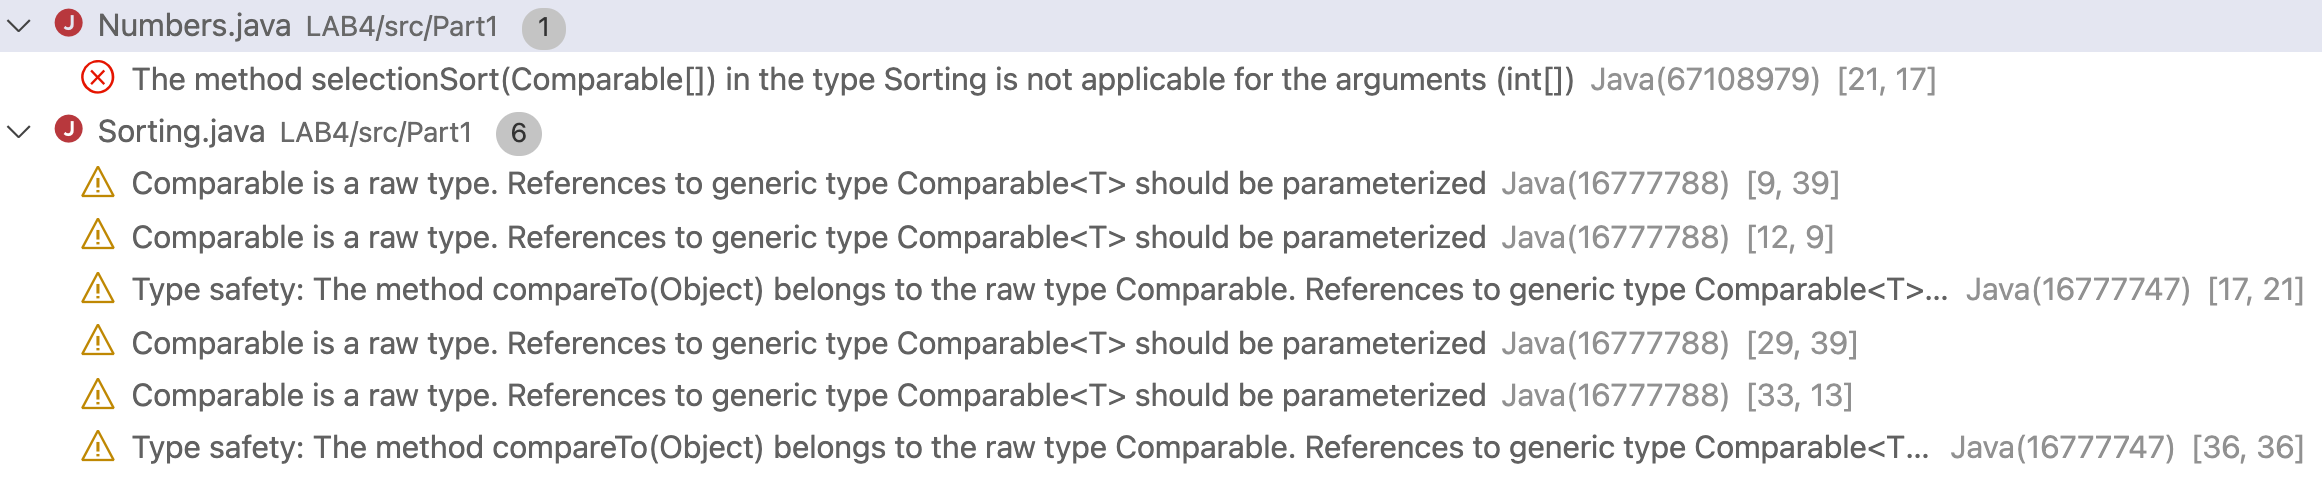
\includegraphics[scale=0.4]{numbers_error.png} 


\begin{itemize}
    \item[] 
\end{itemize}
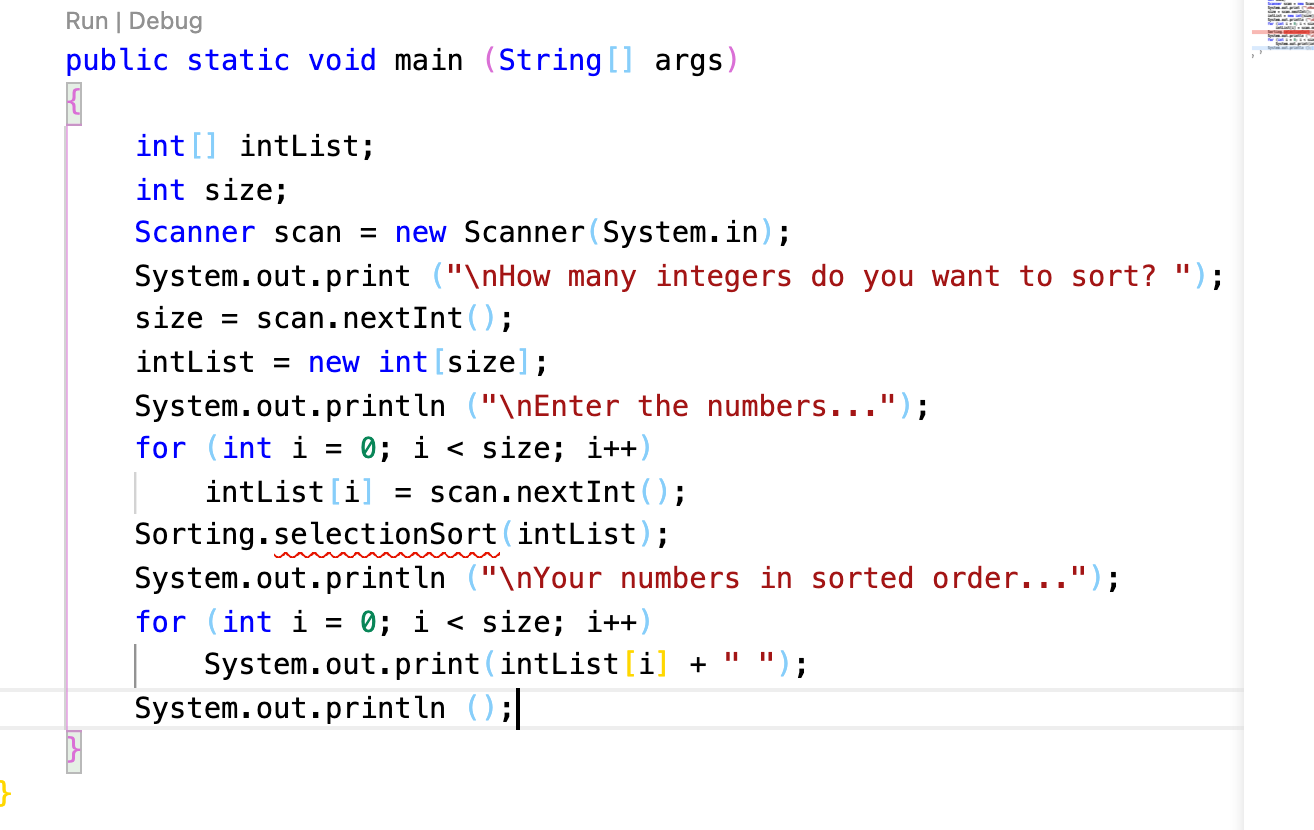
\includegraphics[scale=0.35]{NumbersBef.png}
$\longrightarrow$ 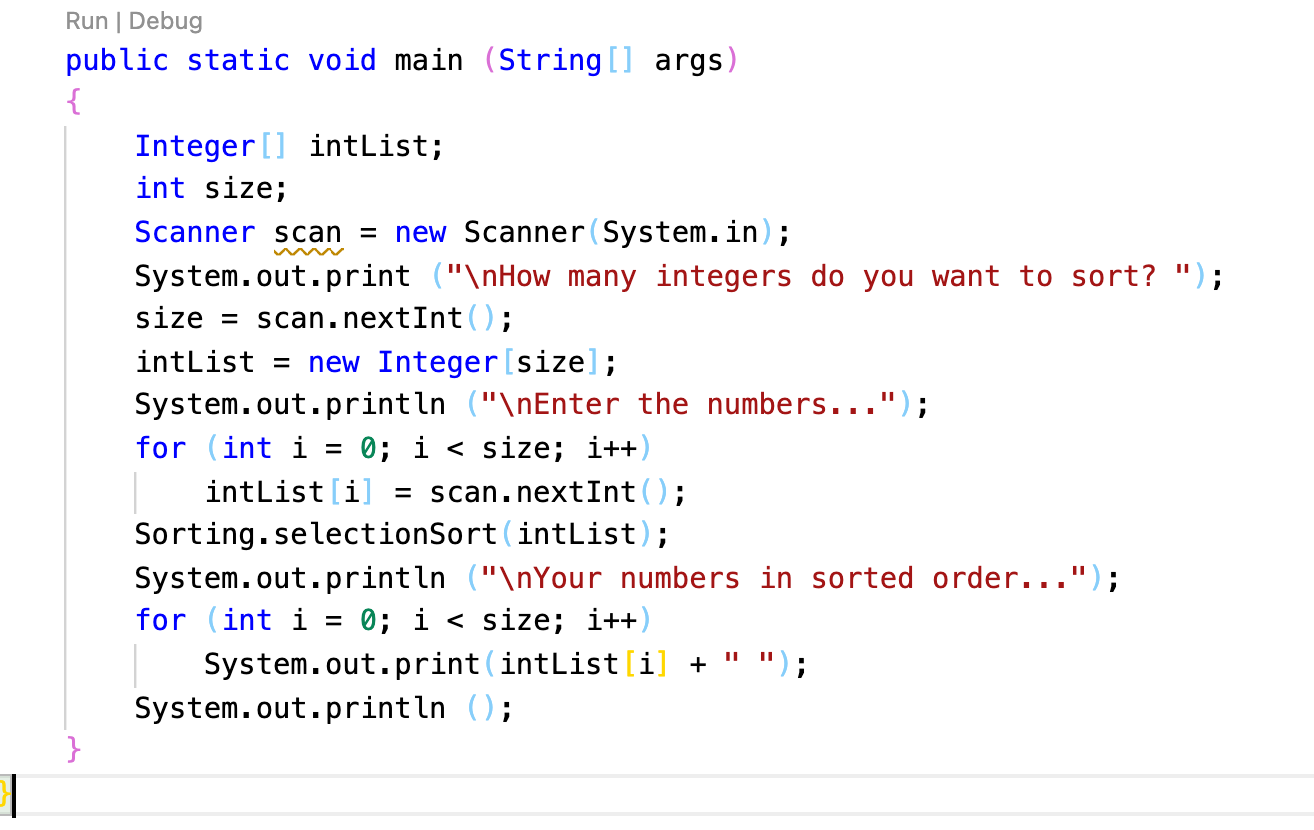
\includegraphics[scale=0.35]{NumbersCode.png}
\\ 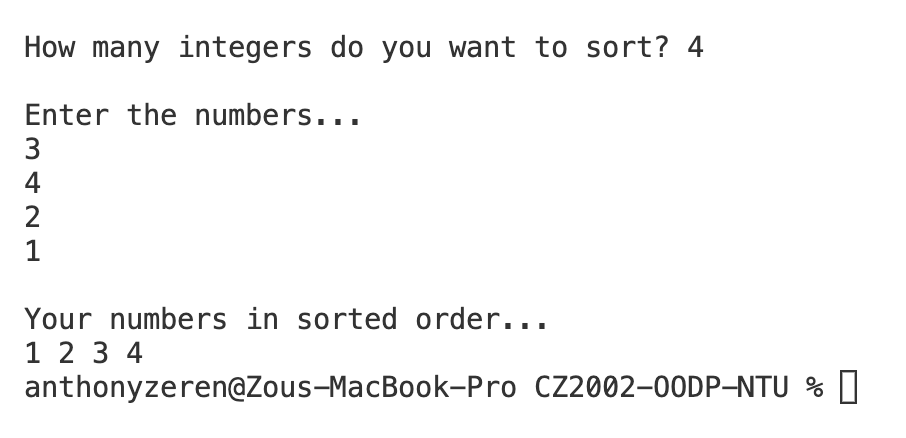
\includegraphics[scale=0.6]{NumbersResult.png}

\section{String.java}
\textit{Write a program Strings.java, similar to Numbers.java, that reads in an array of String objects and sorts
them. You may just copy and edit Numbers.java.}

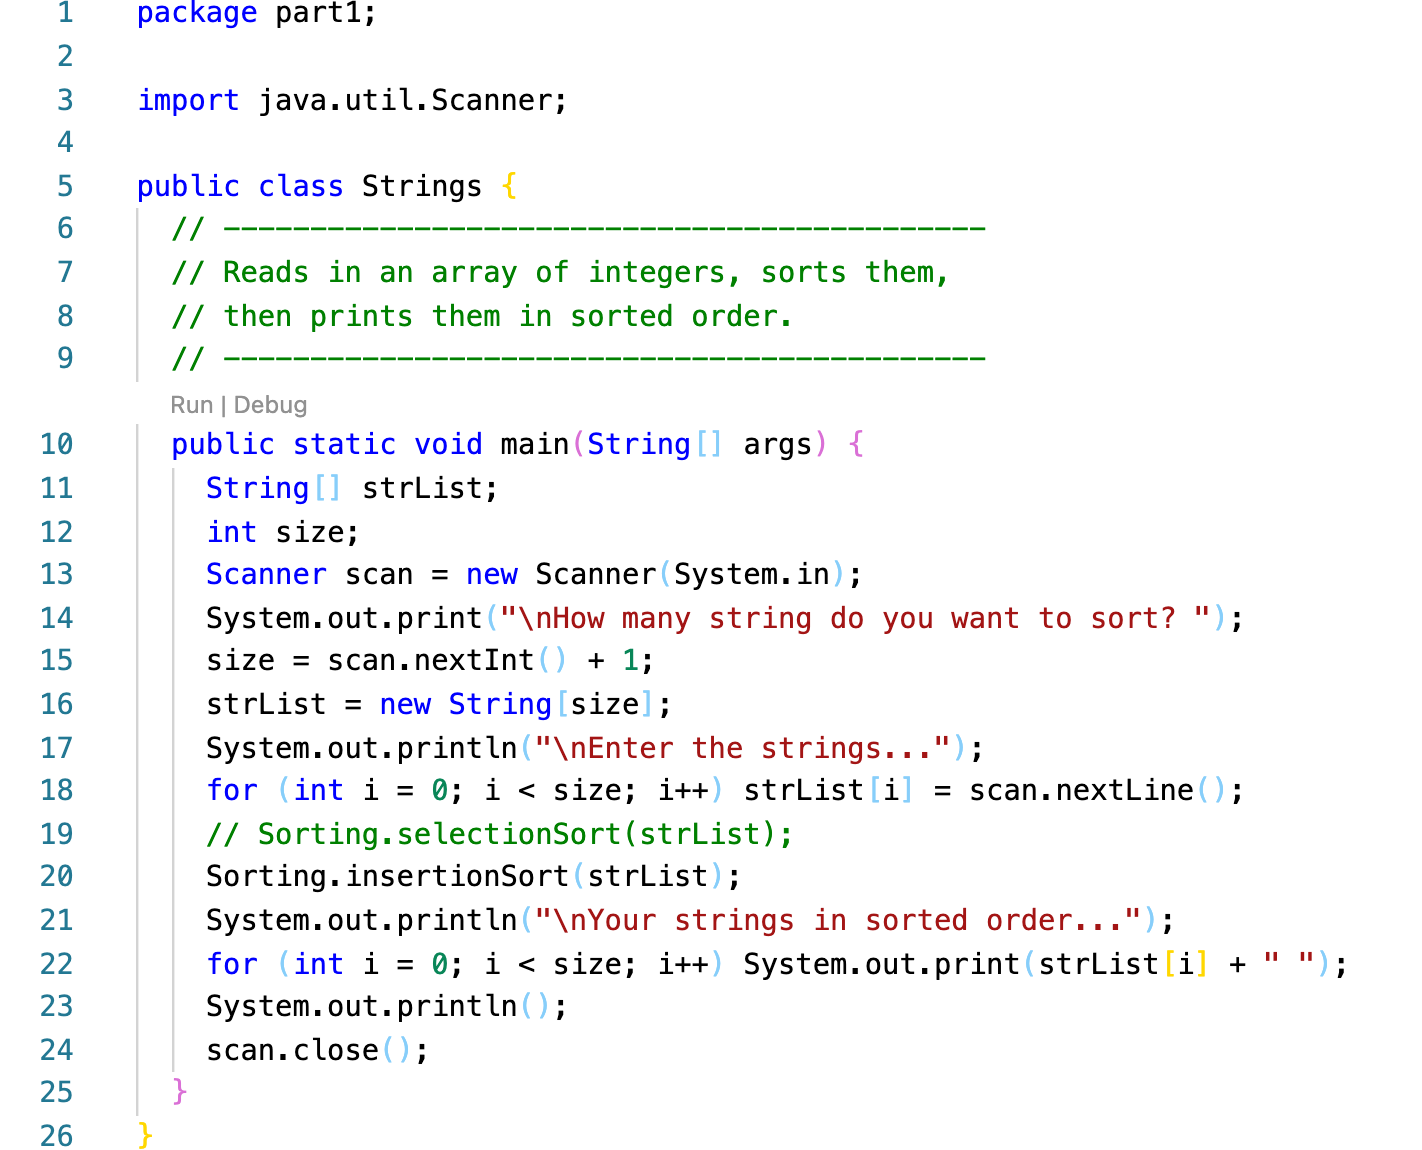
\includegraphics[scale=0.4]{StringCode.png}
$\longrightarrow$ 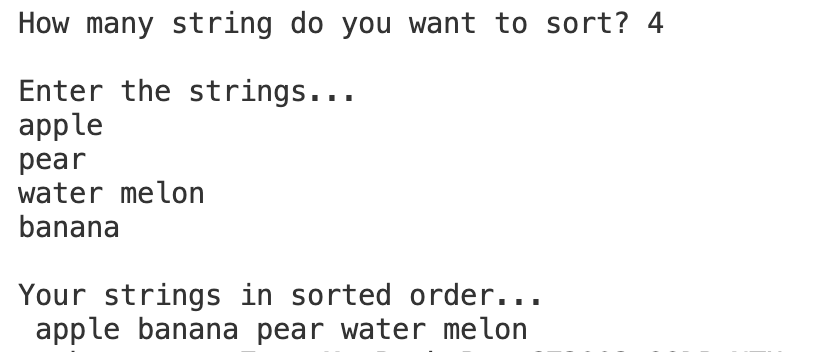
\includegraphics[scale=0.5]{StringsResult.png}

\section{Decending Insertion Sort}
\textit{Modify the insertionSort algorithm so that it sorts in descending order rather than ascending order.
Change Numbers.java and Strings.java to call insertionSort rather than selectionSort. Run both to make
sure the sorting is correct.}
Decending Insertion Sort \qquad\qquad\qquad\qquad\qquad\quad Tested on Numbers

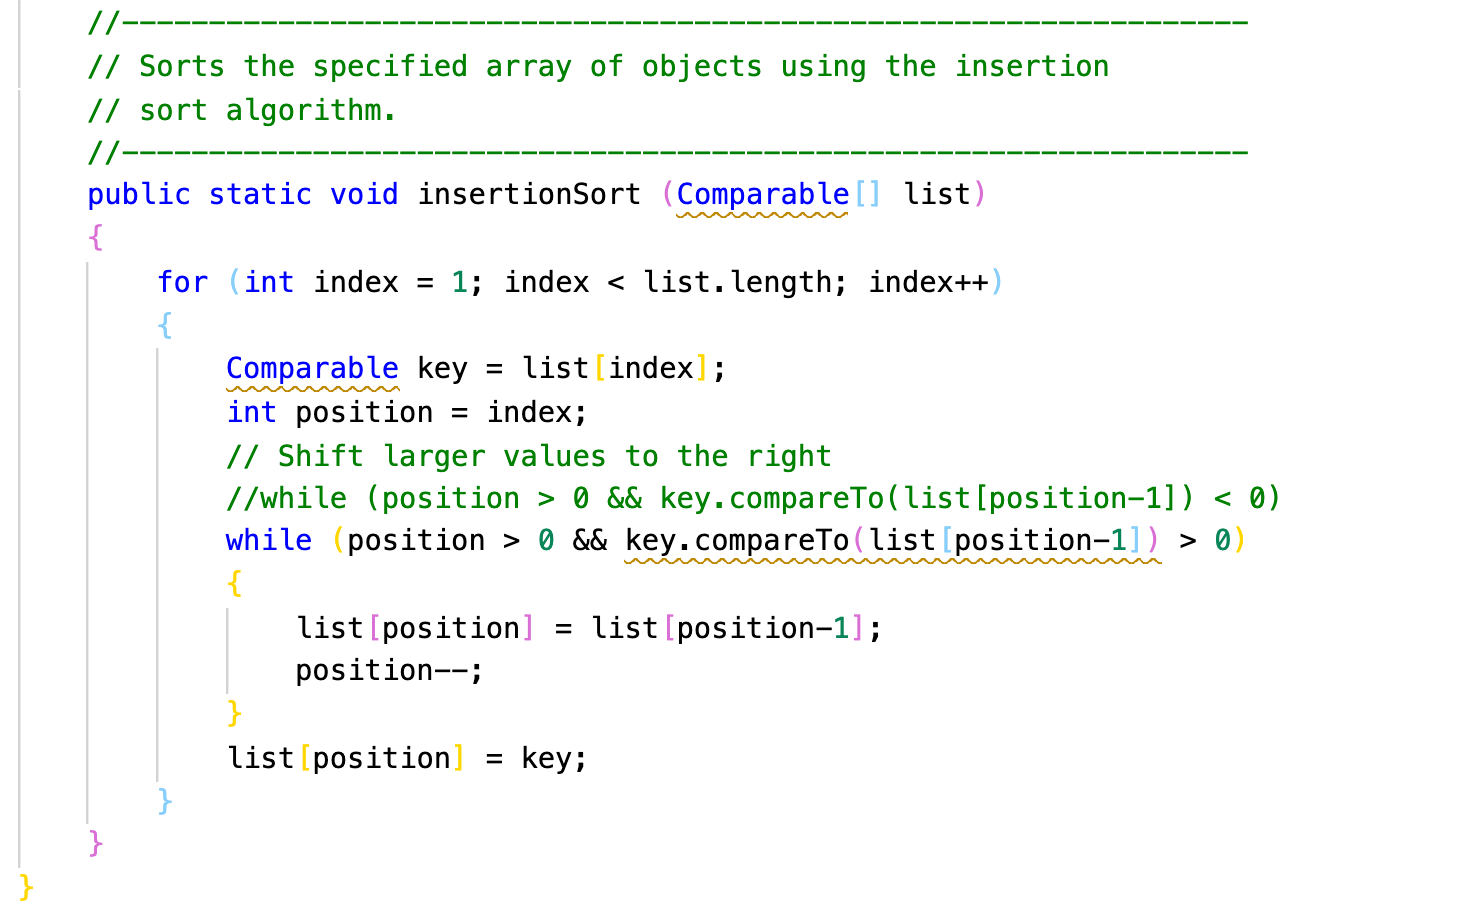
\includegraphics[scale=0.35]{desInsert.png} 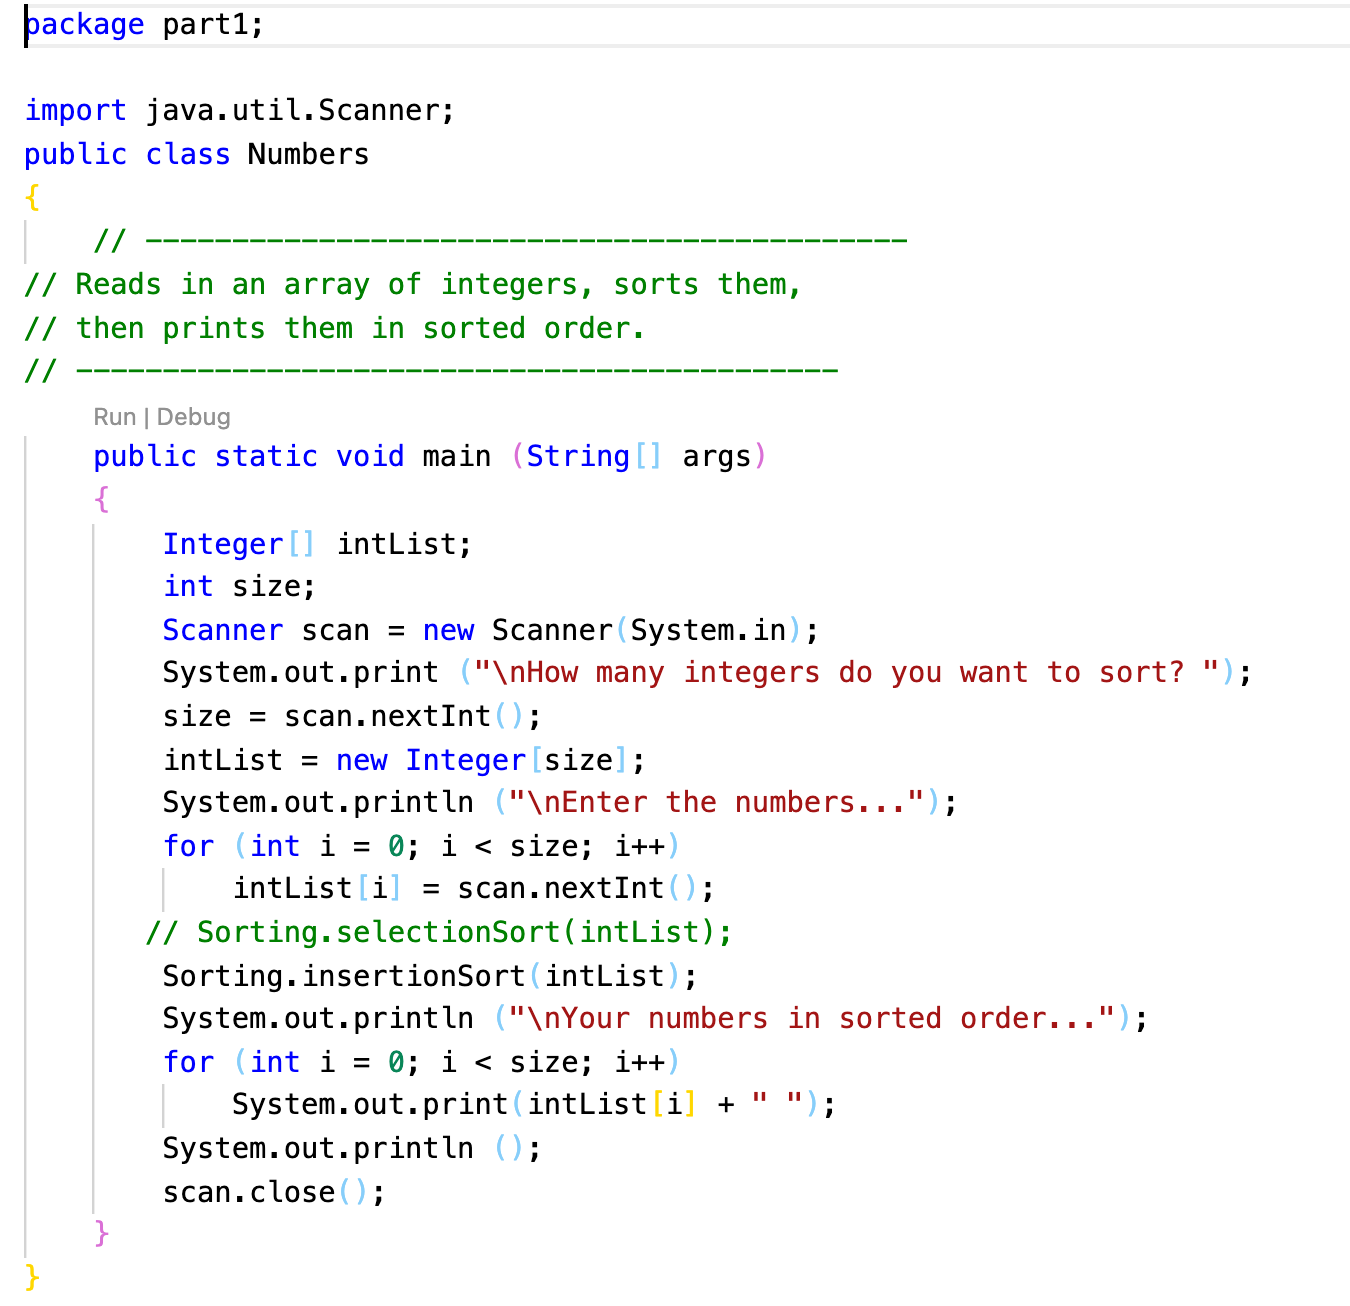
\includegraphics[scale=0.35]{newNum.png}

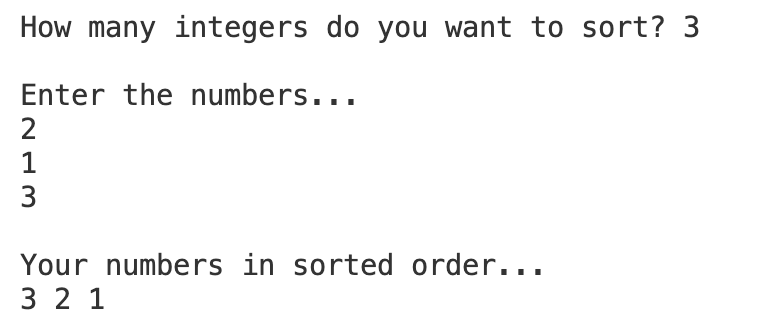
\includegraphics[scale=0.55]{newNumR.png}

Tested on Strings

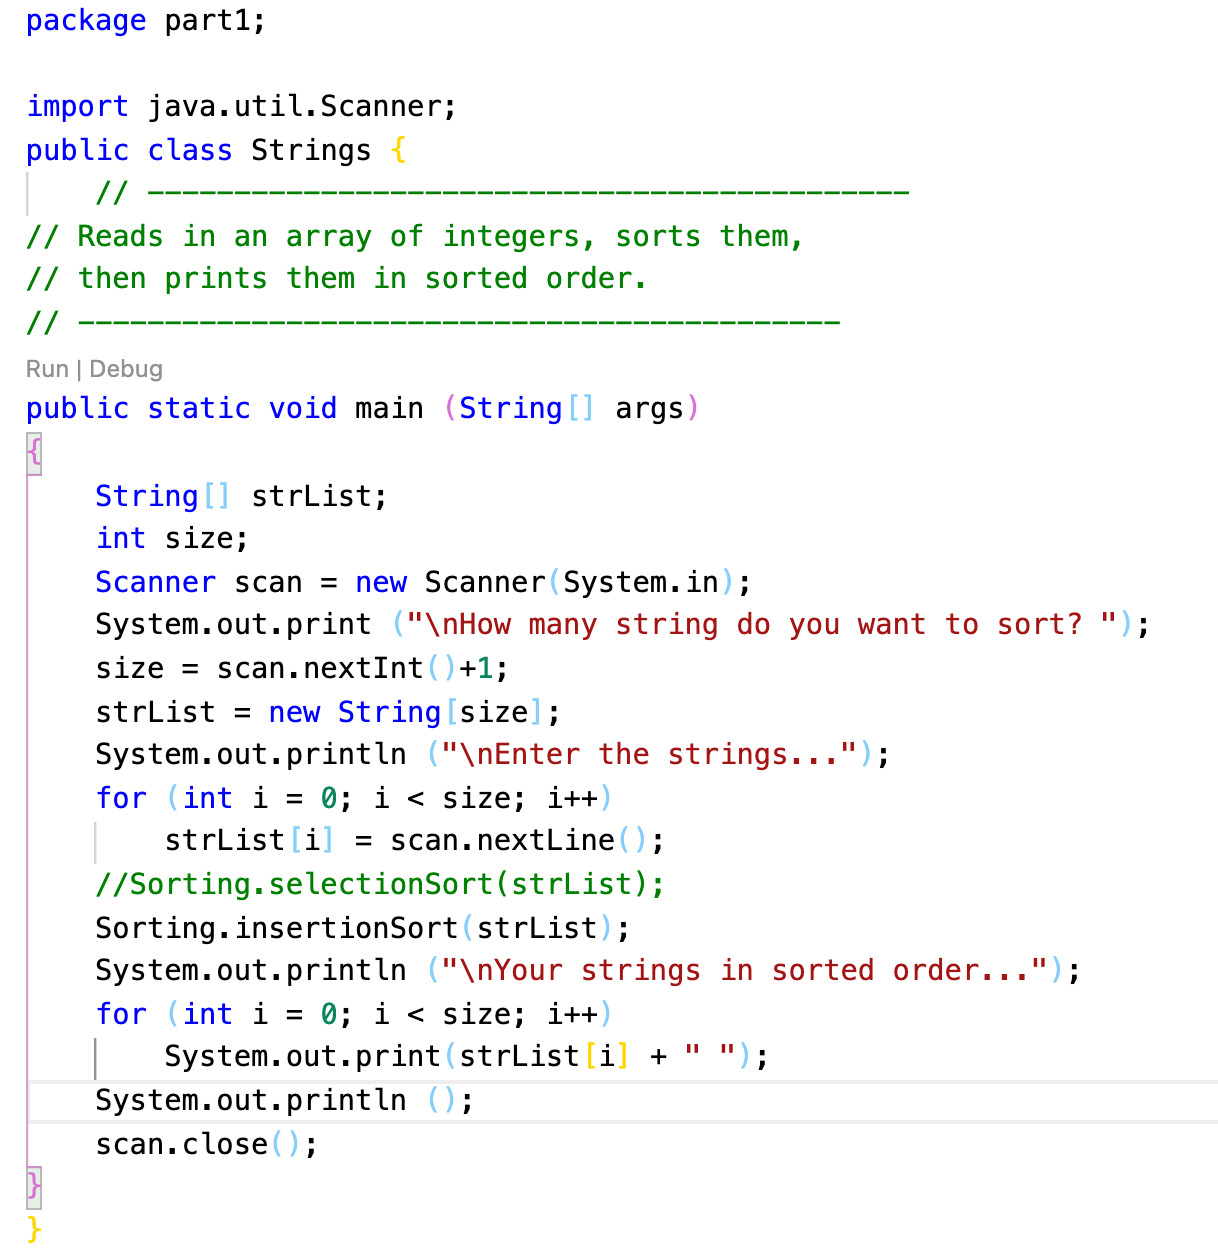
\includegraphics[scale=0.4]{newStrings.png}
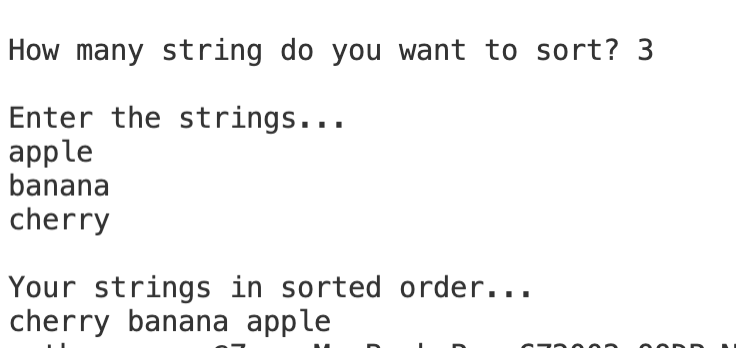
\includegraphics[scale=0.55]{newStringR.png}

\newpage
\section{SalesPerson Class}
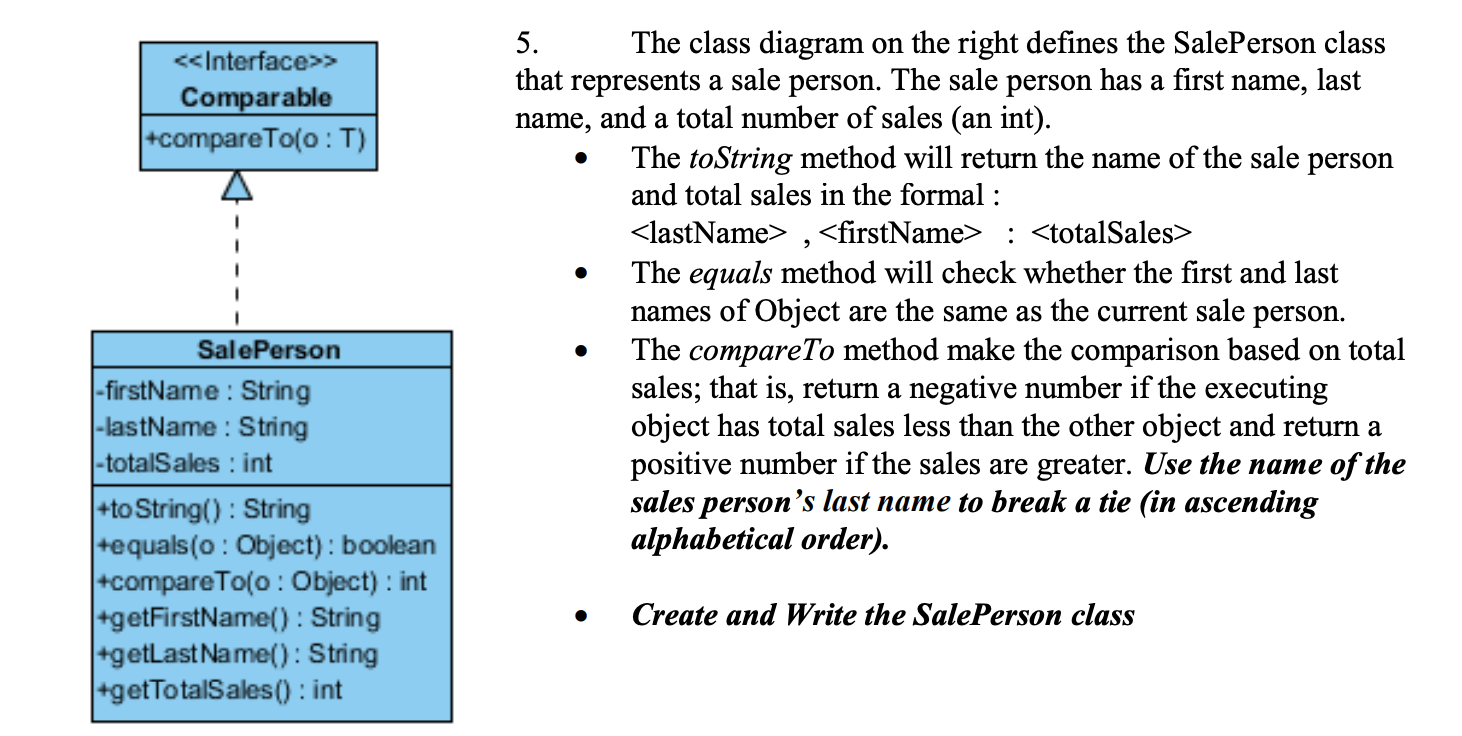
\includegraphics[scale=0.55]{q5.png} 

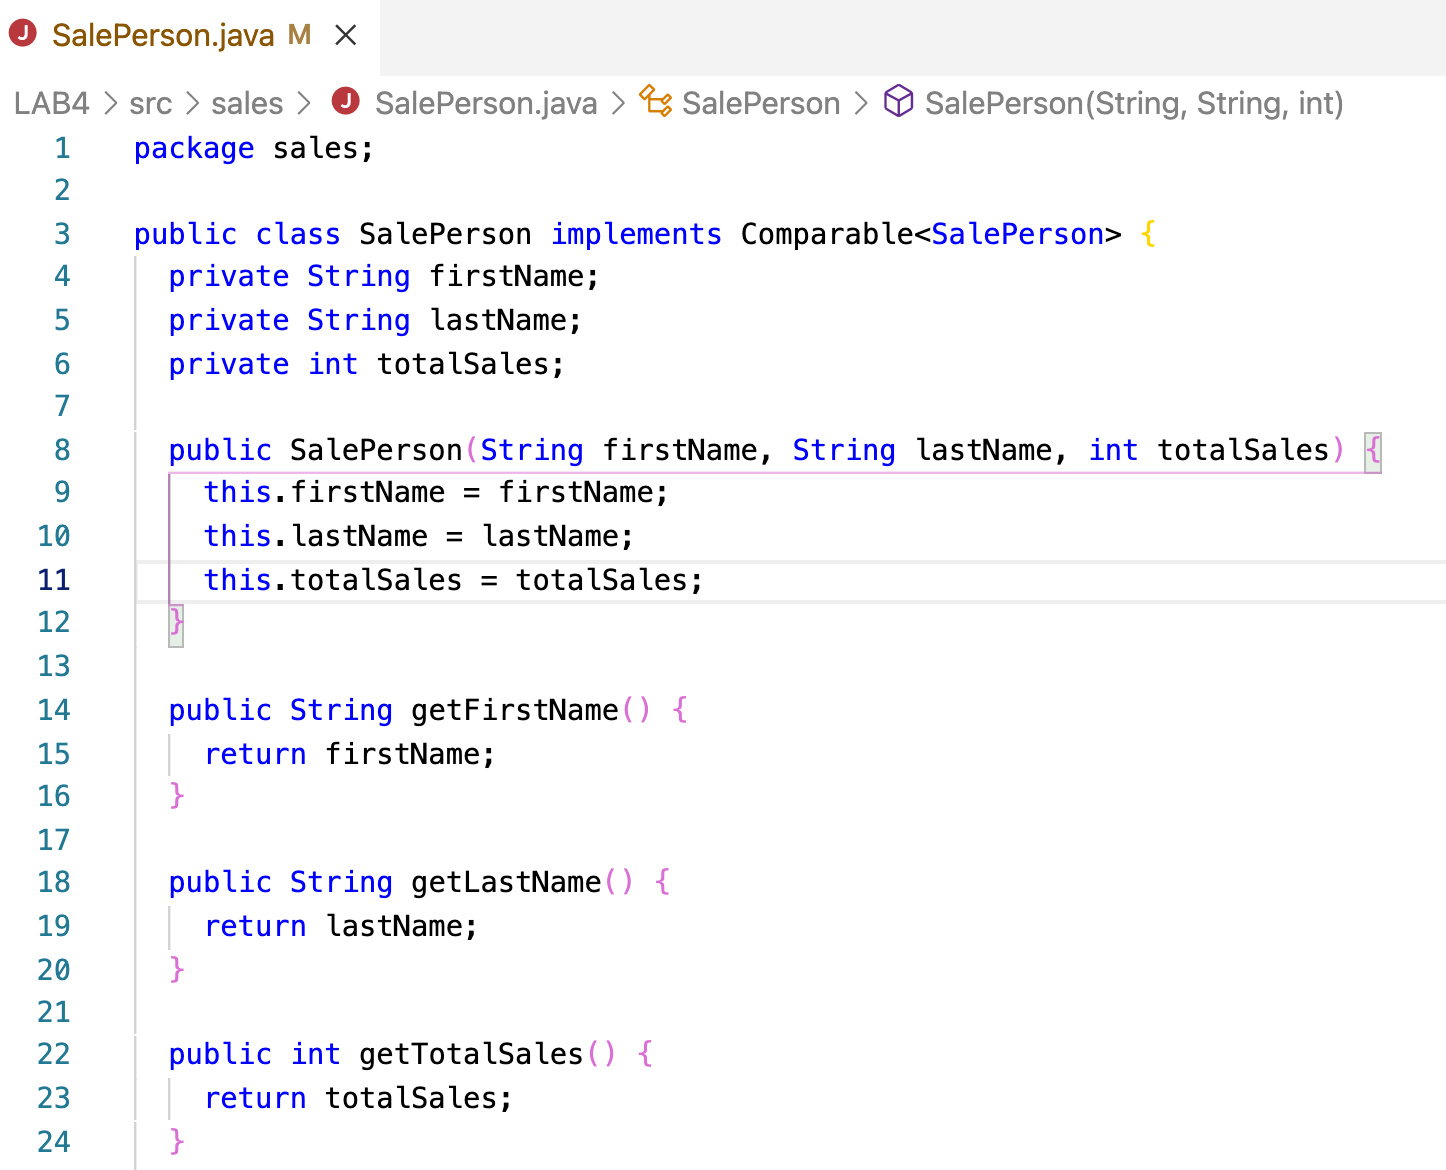
\includegraphics[scale=0.3]{SalesPerson1.png}
\quad
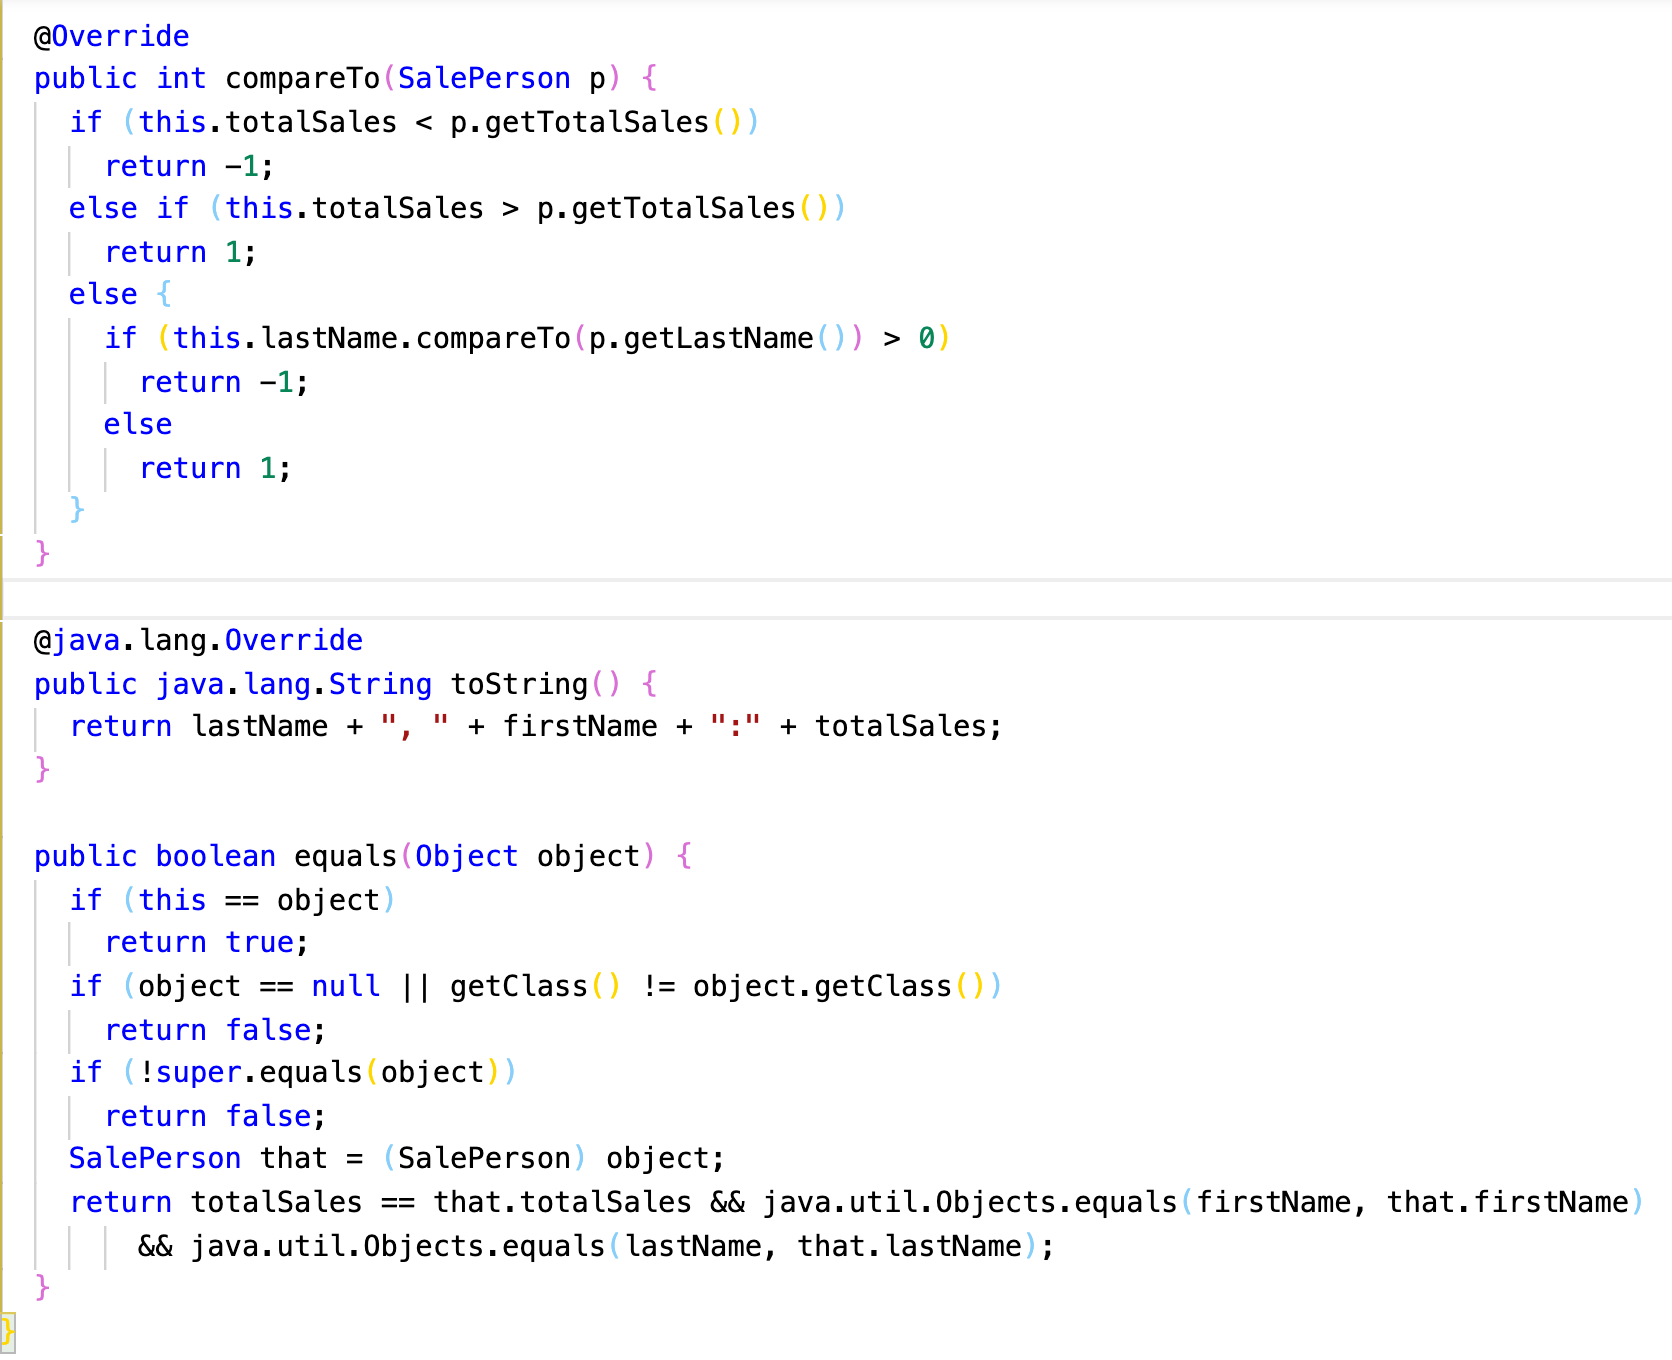
\includegraphics[scale=0.25]{SalesPerson2.png}
\newpage

\section{WeeklySales}
\textit{The file WeeklySales.java (in attachment) contains a driver for testing the compareTo method and the
sorting . Compile and run it. Make sure your compareTo method is correct. The sales staff should be
listed in the order of sales from most to least. If the sale staffs have the same number of sales, they
are listed in ascending alphabetical order of their last names.}'

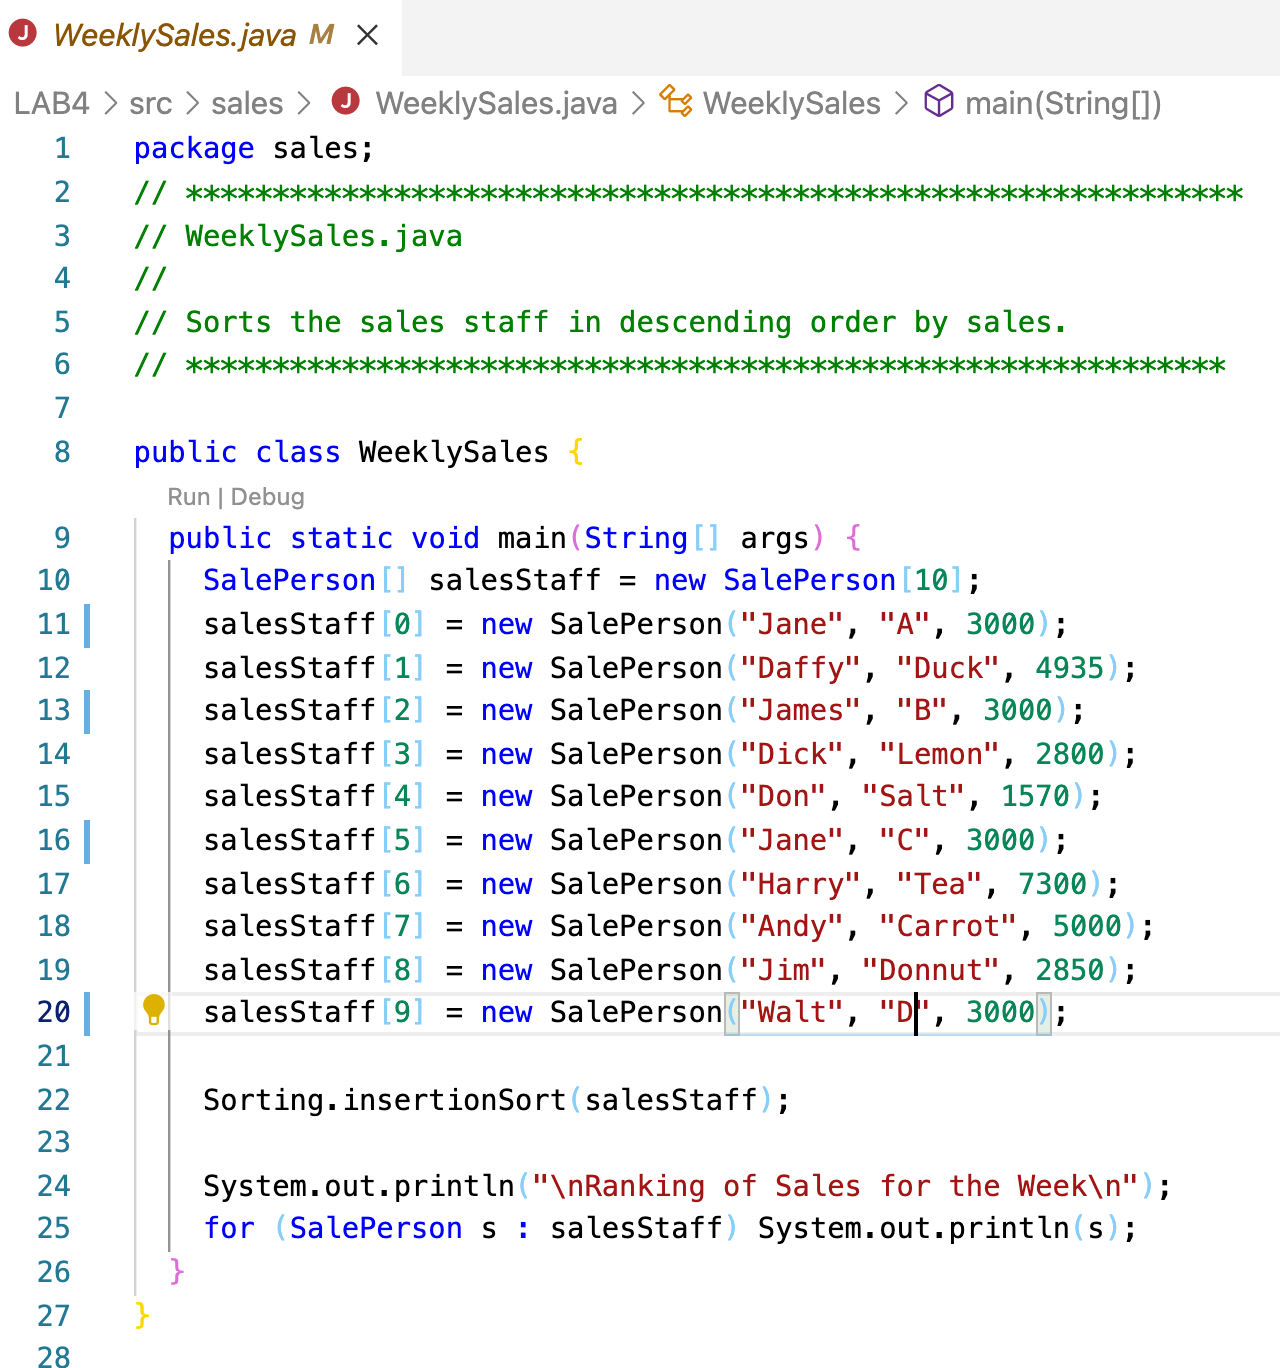
\includegraphics[scale=0.35]{WeeklySalesCode.png}
$\longrightarrow$ 
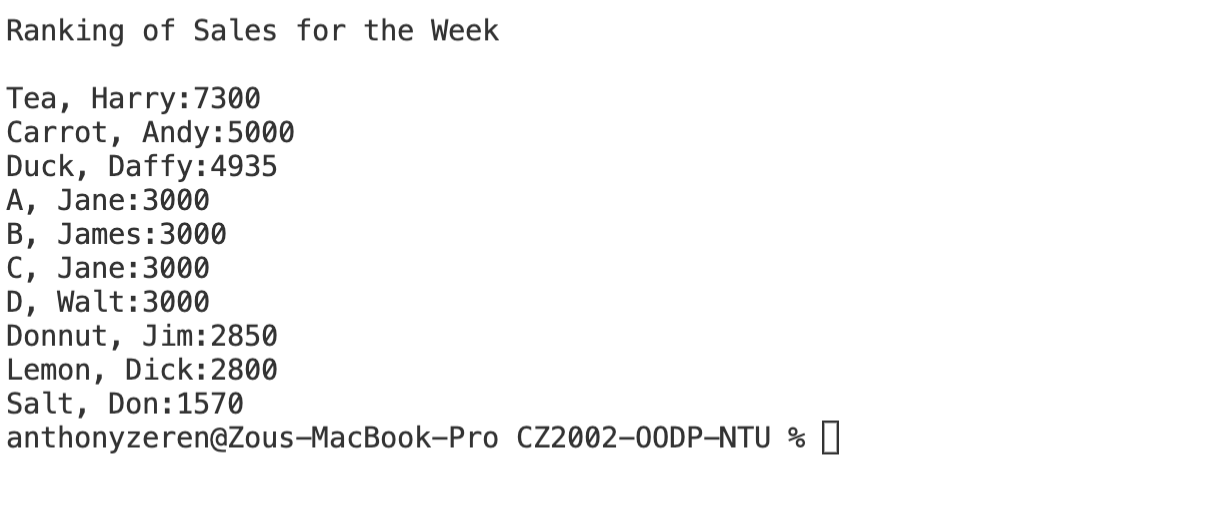
\includegraphics[scale=0.4]{WeeklySalesResult.png}

\section{Calculate Surface Area of a Figure}

\textit{
\begin{enumerate}
\item[] 
By using the concepts of inheritance and polymorphism, you are required to design a program that
calculate the total surface area of a figure. The following are the requirements an constraints :
\item[]  You should have a Class/Interface called Shape and decide its appropriate attributes and
behaviours
\item [] You should have basic shapes like Square, Rectangle, Circle and Triangle.
\item [] The program will request the user to :
\begin{itemize}
    \item  enter the total number of shapes
    \item choose the shape and enter the required dimension/s for the selected shape
    \item choose the type of calculation (for now, we will just calculate Area, with future plan
    to calculate Volume as well).
\end{itemize}
\item [] The calculation/s should be done upon user’s request and NOT when dimensions are entered.
\item For a start, use the 2-D figure on the right to verify your program. The figure
consists of a Circle (radius=10), a Triangle (height=25, base =20) and a Rectangle
(length=50, breadth = 20) . Calculate the total area of the 2- D figure.
(You will create an Application class Shape2DApp.java for this purpose)
\item  We will now expand and extend your design to cater to 3-D figures. Imagine the
figure on the right is turn into a 3-D figure – Circle becomes Sphere, Triangle
becomes a square-based Pyramid and the Rectangle is a cubiod. Calculate the
total surface area of the 3- D figure. [Note : You need to think whether ‘is a’ or
‘has a’ relationship is more appropriate and relevant for between 2D and 3D
shapes.
(You will create an Application class Shape3DApp.java for this purpose)
\item  We will include more Shapes. The square-based Pyramid will be replaced with a
Cone and the Cubiod is replaced with a Cylinder. Calculate the total surface area
of the new 3- D figure.
(You will reuse the Application class Shape3DApp.java with appropriate
selection)
\end{enumerate}
}

    \subsection{shape.java}
    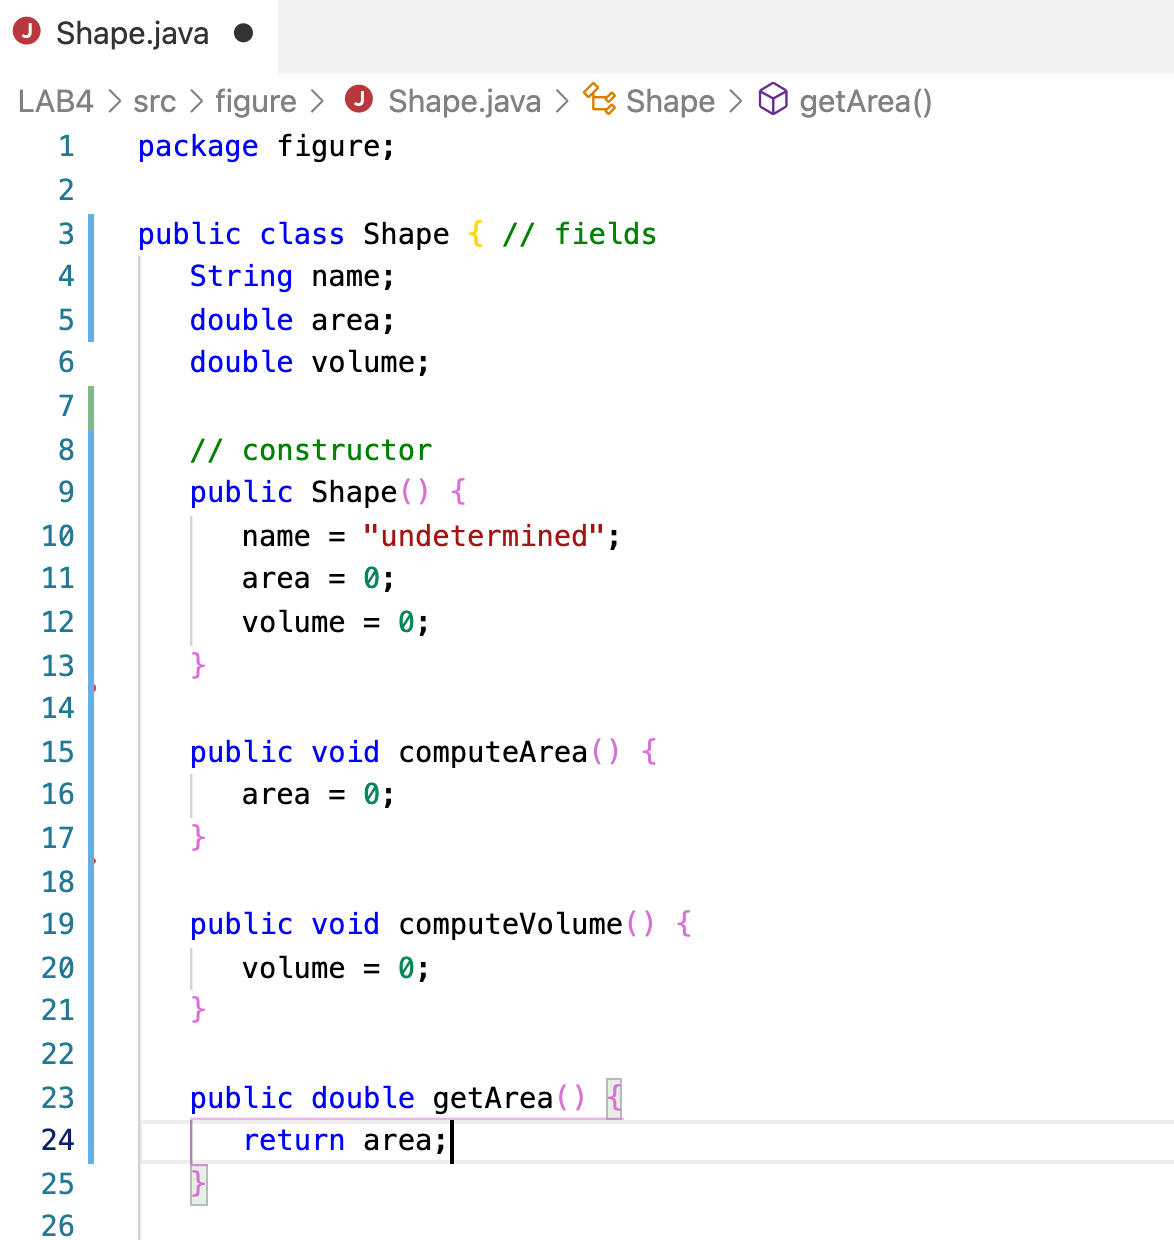
\includegraphics[scale=0.4]{z_shape1.png}
    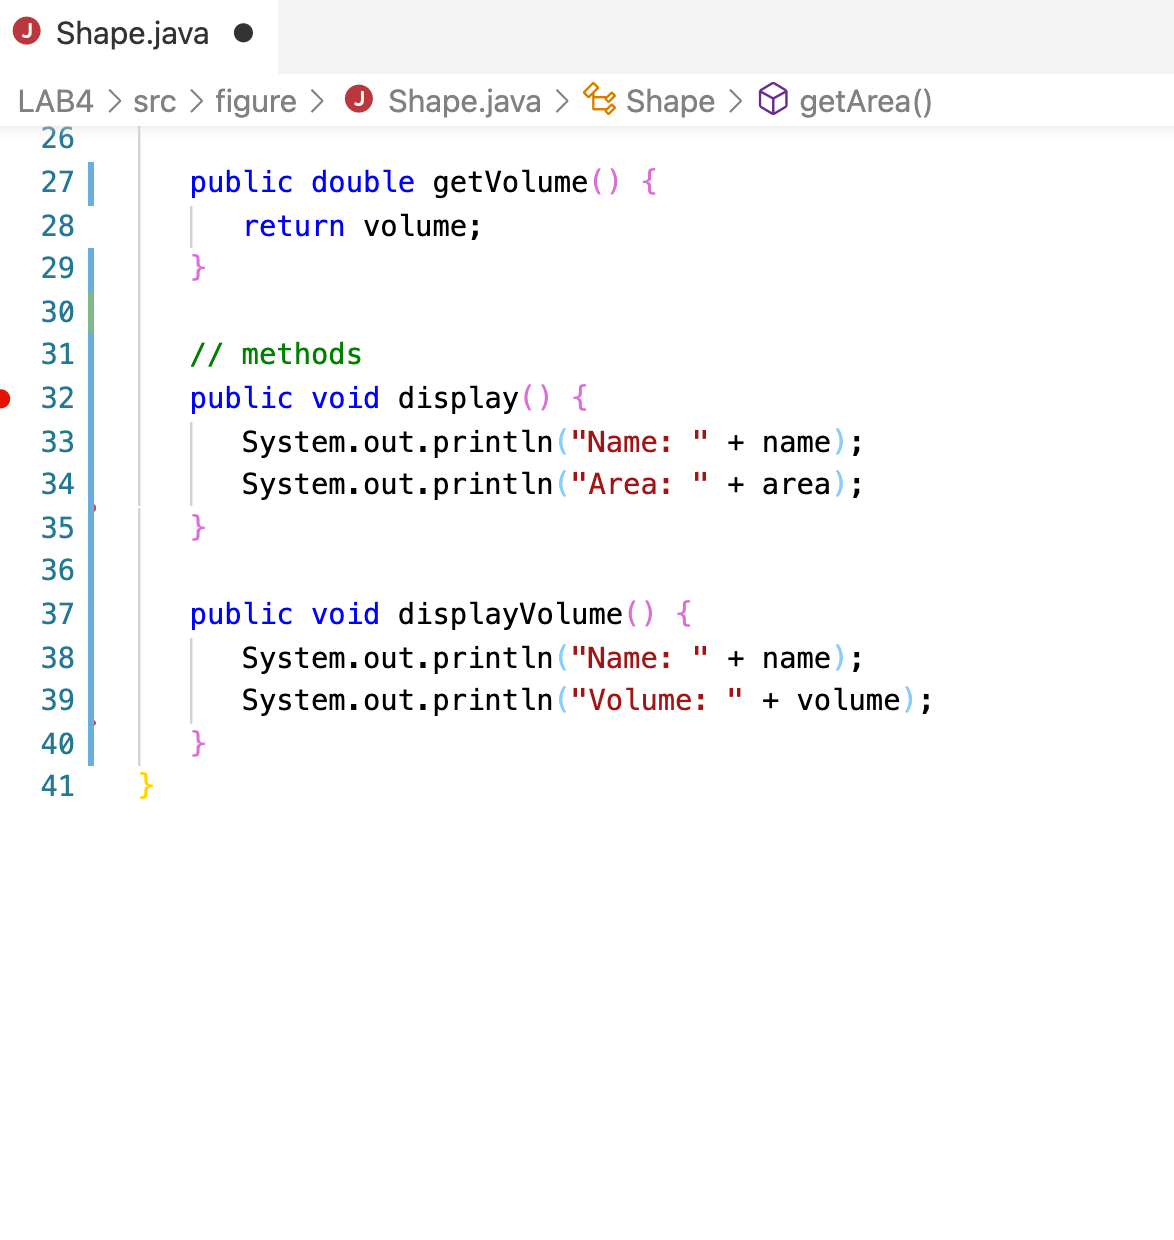
\includegraphics[scale=0.4]{z_shape2.png}
    
    \subsection{Cirle.java}
    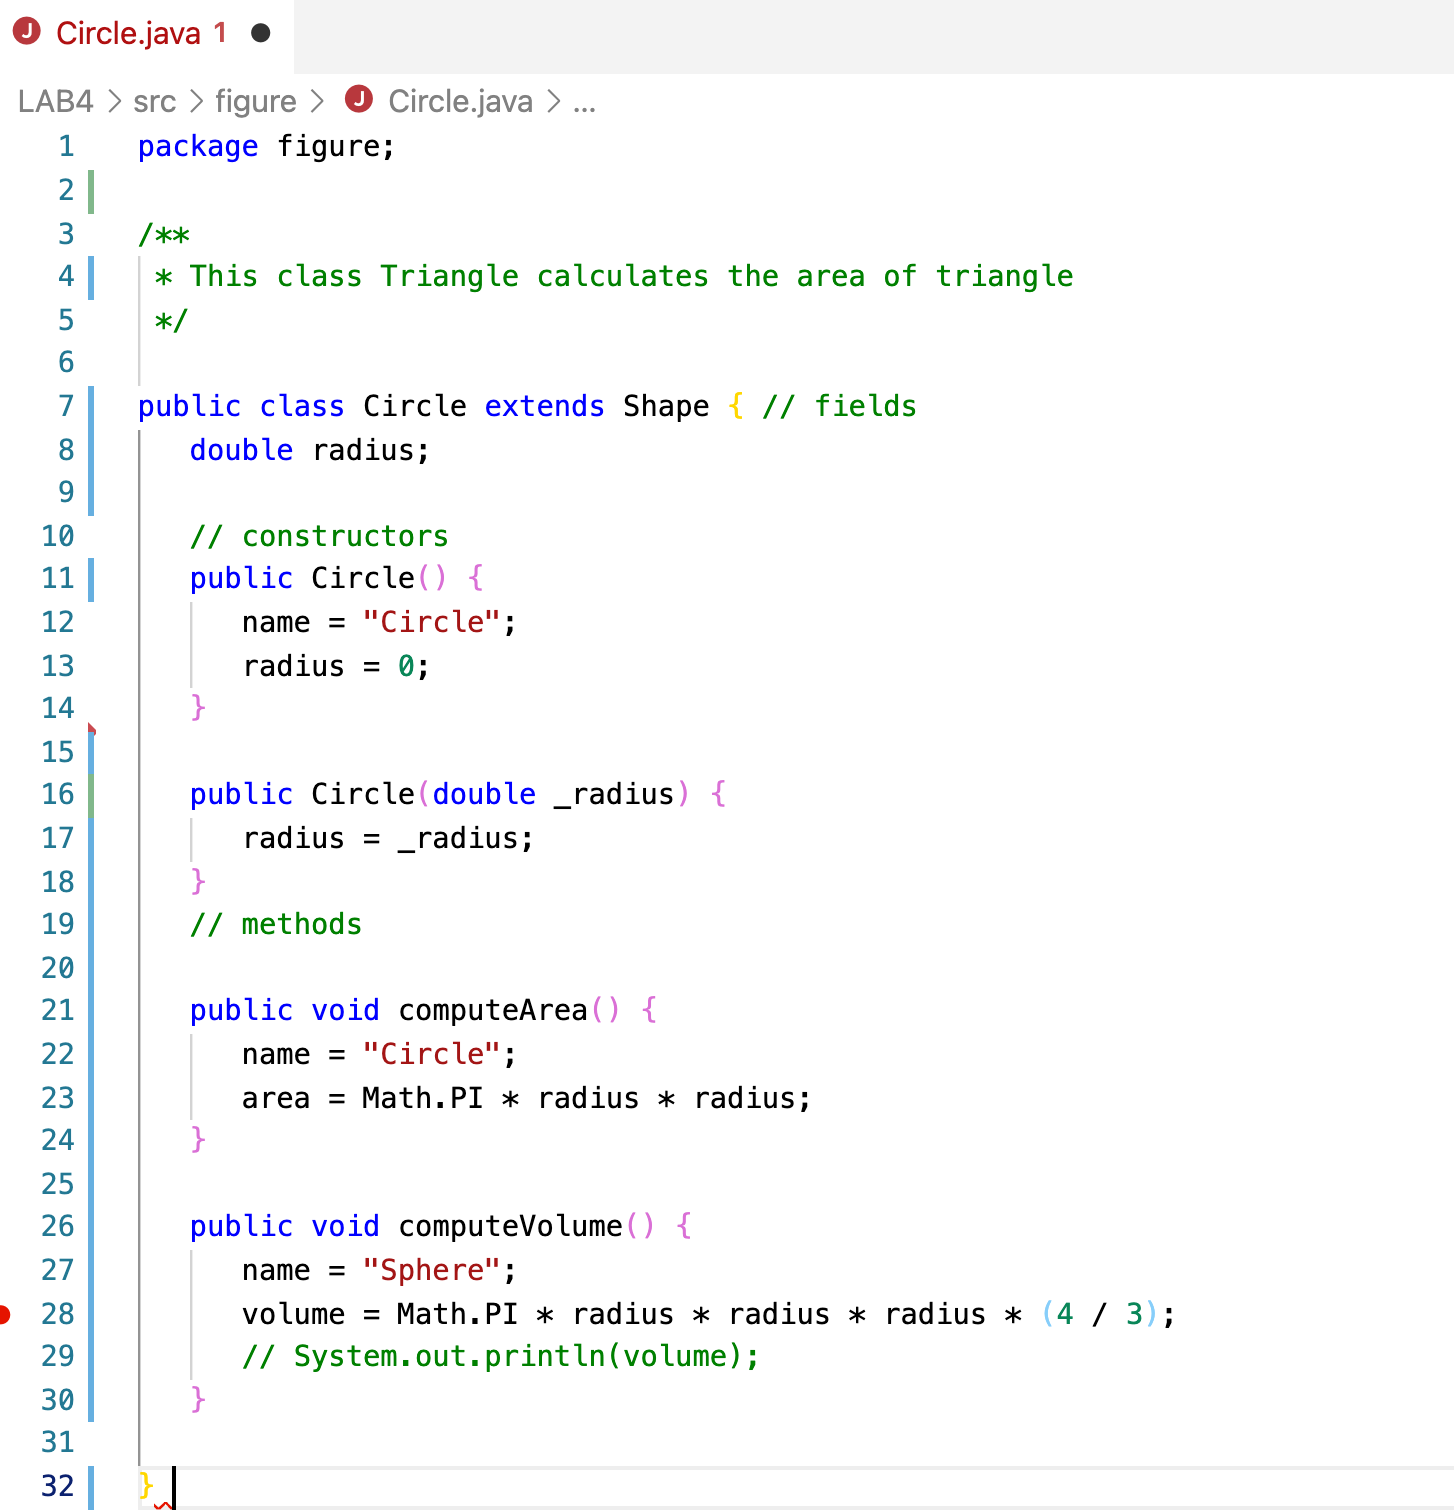
\includegraphics[scale=0.4]{z_circle.png}
    
    
    \subsection{Square.java}
    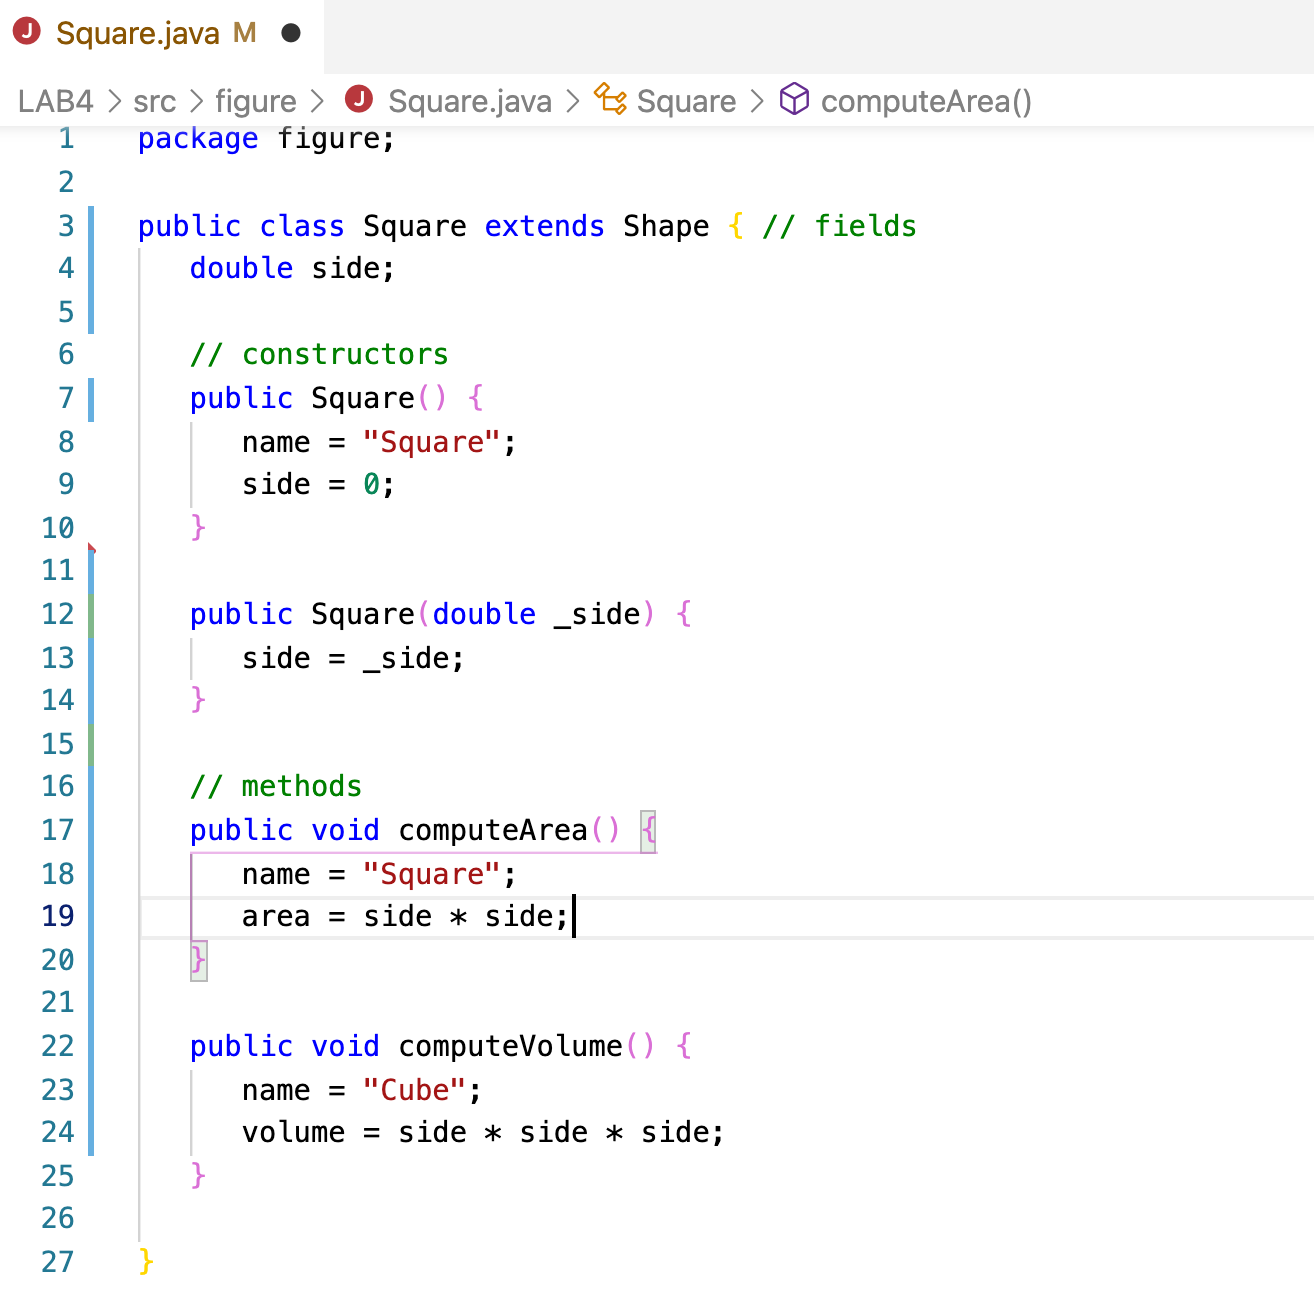
\includegraphics[scale=0.4]{z_square.png}
    
    
    \subsection{Rectangle.java}
    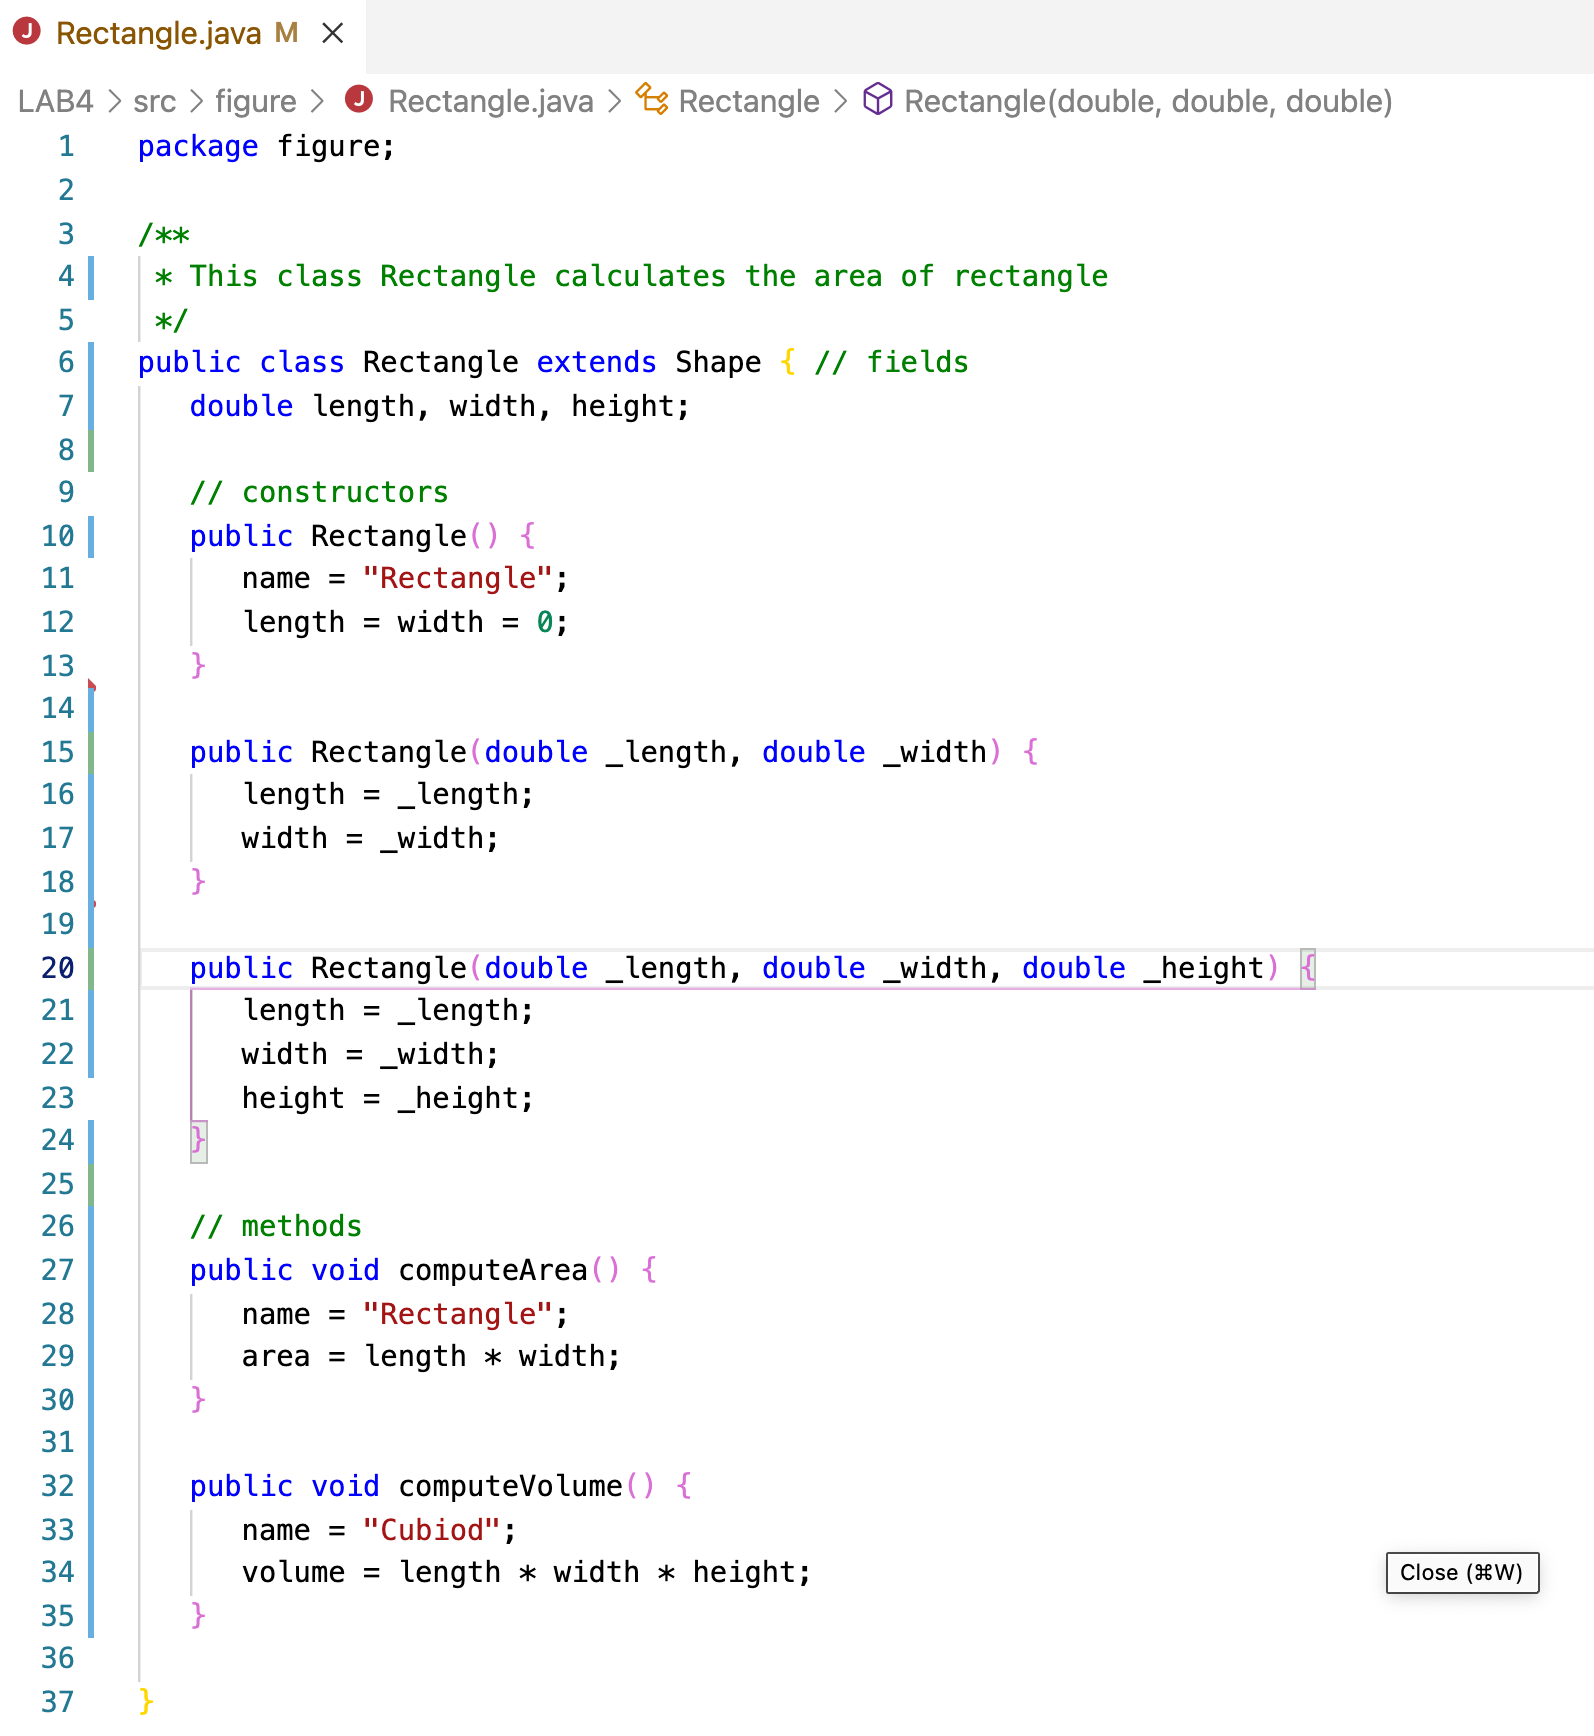
\includegraphics[scale=0.4]{z_rectangle.png}
    
    
    \subsection{Triangle.java}
    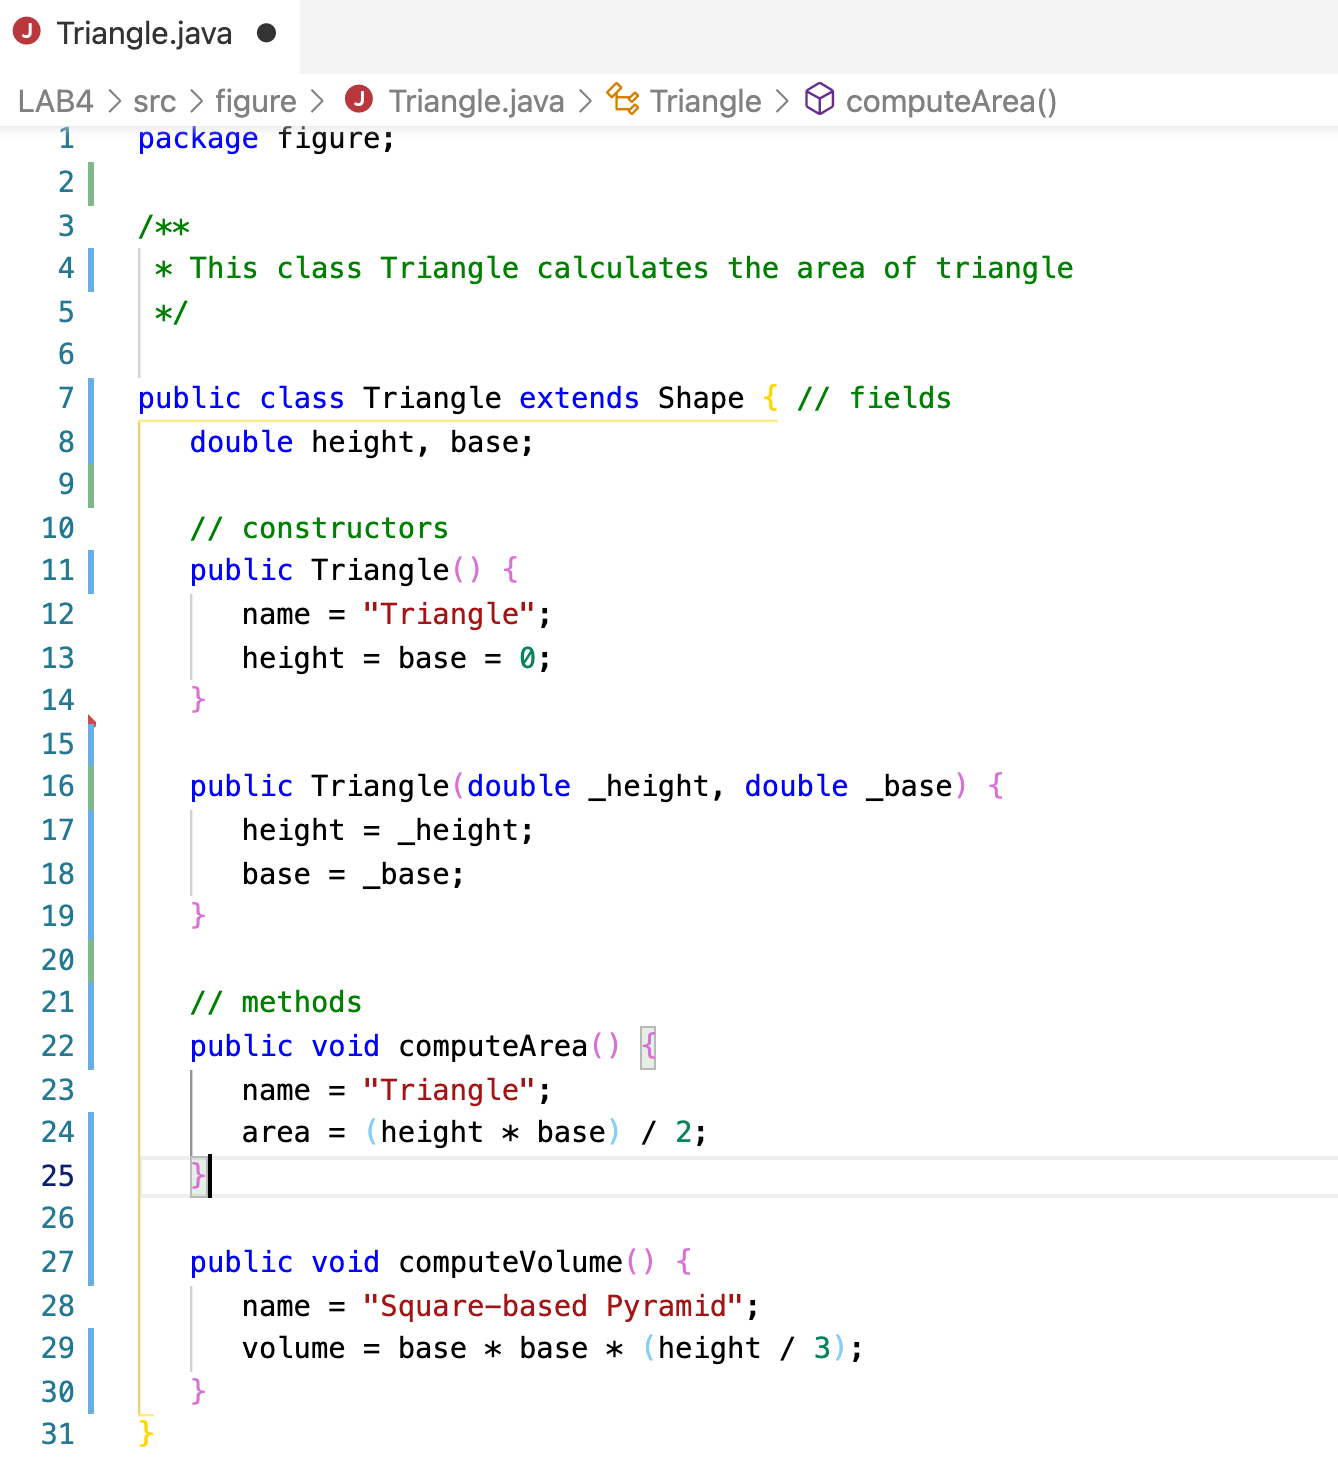
\includegraphics[scale=0.4]{z_triangle.png}
    
    \subsection{Shape2DApp.java}
     
    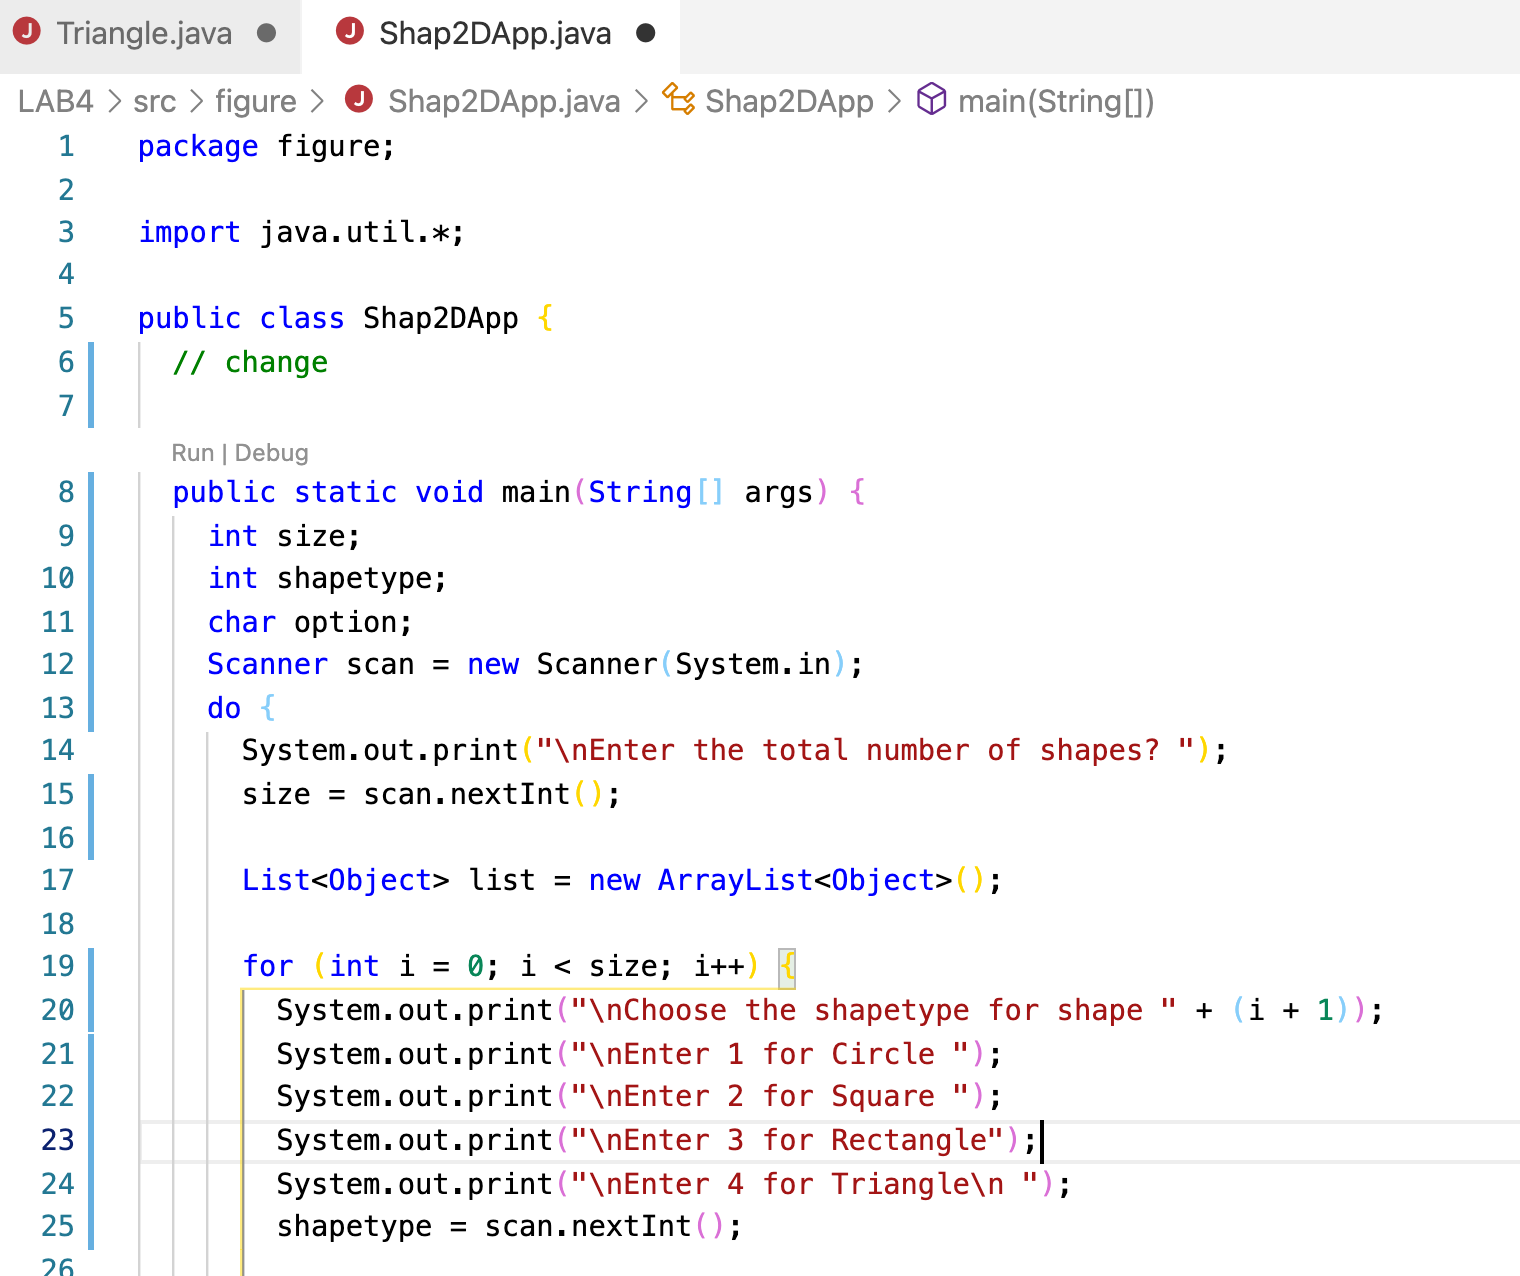
\includegraphics[scale=0.35]{z_shap2dapp1.png}
    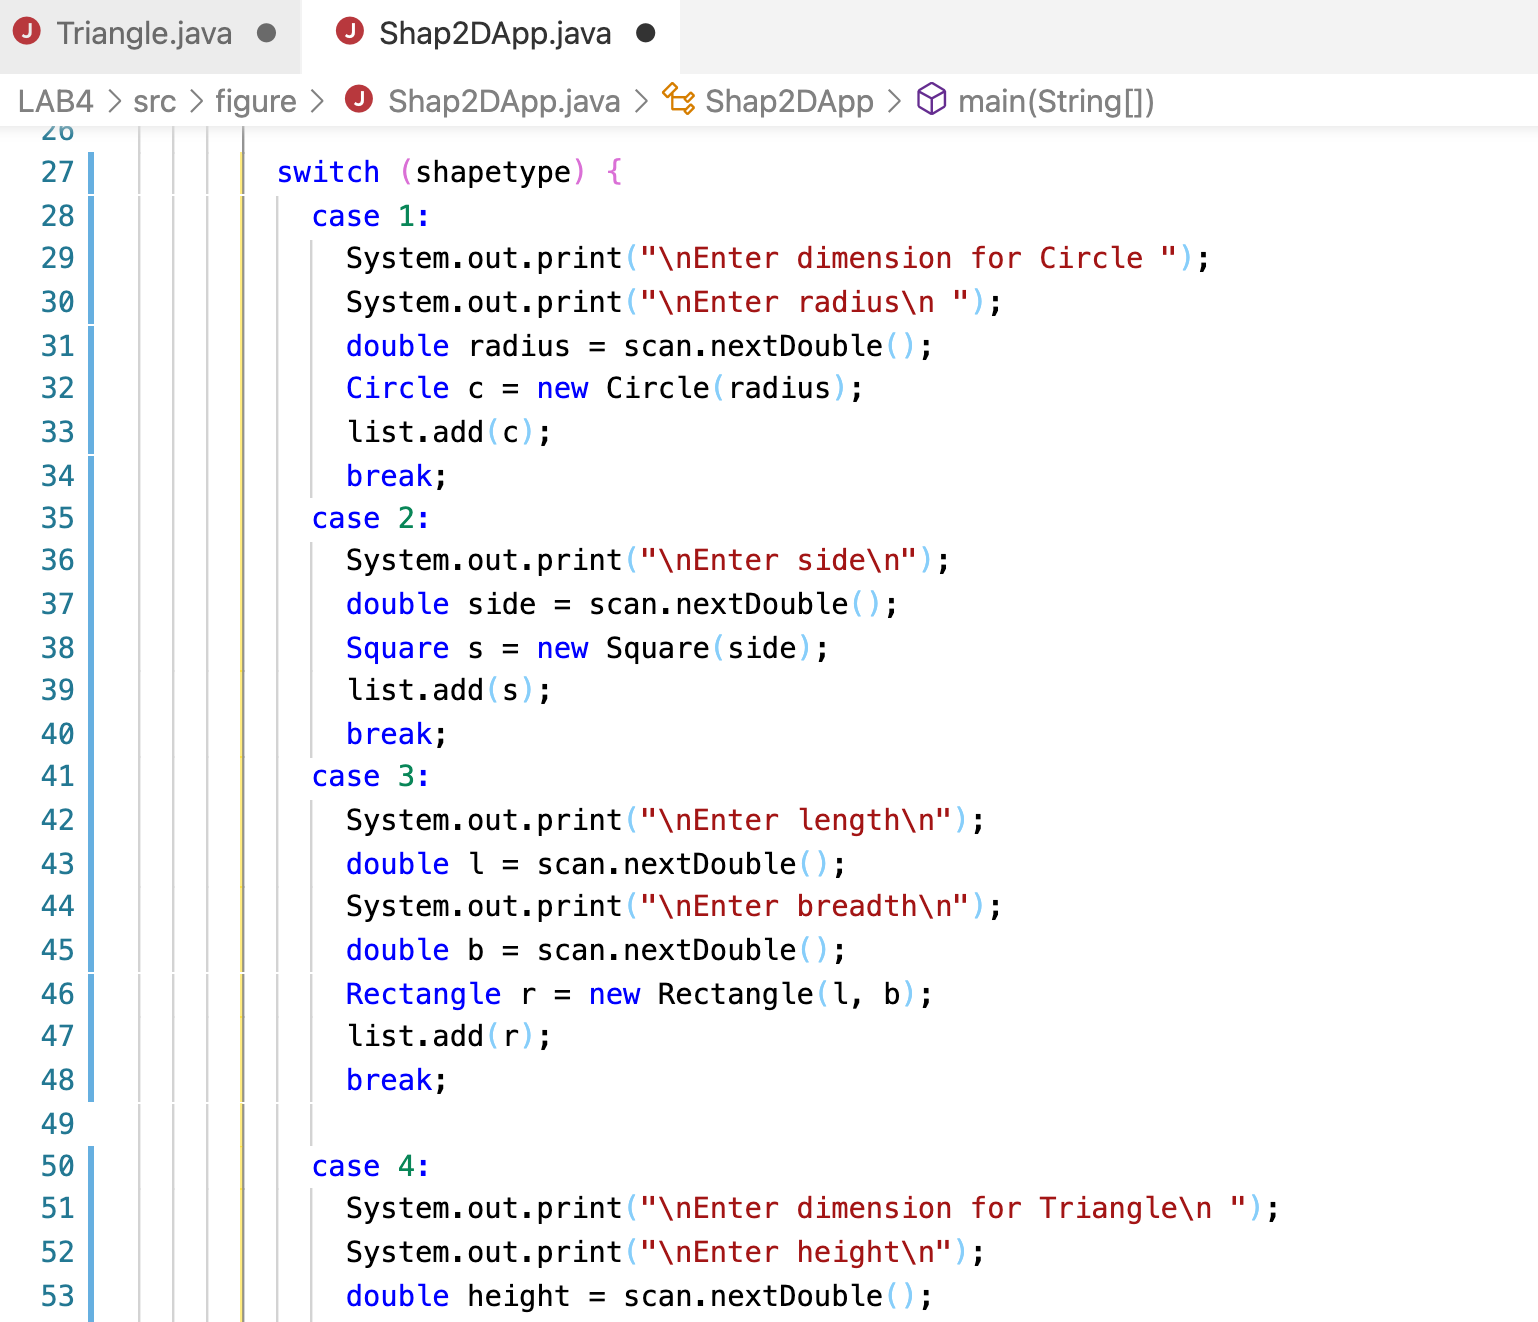
\includegraphics[scale=0.35]{z_shape2dapp2.png}
    
    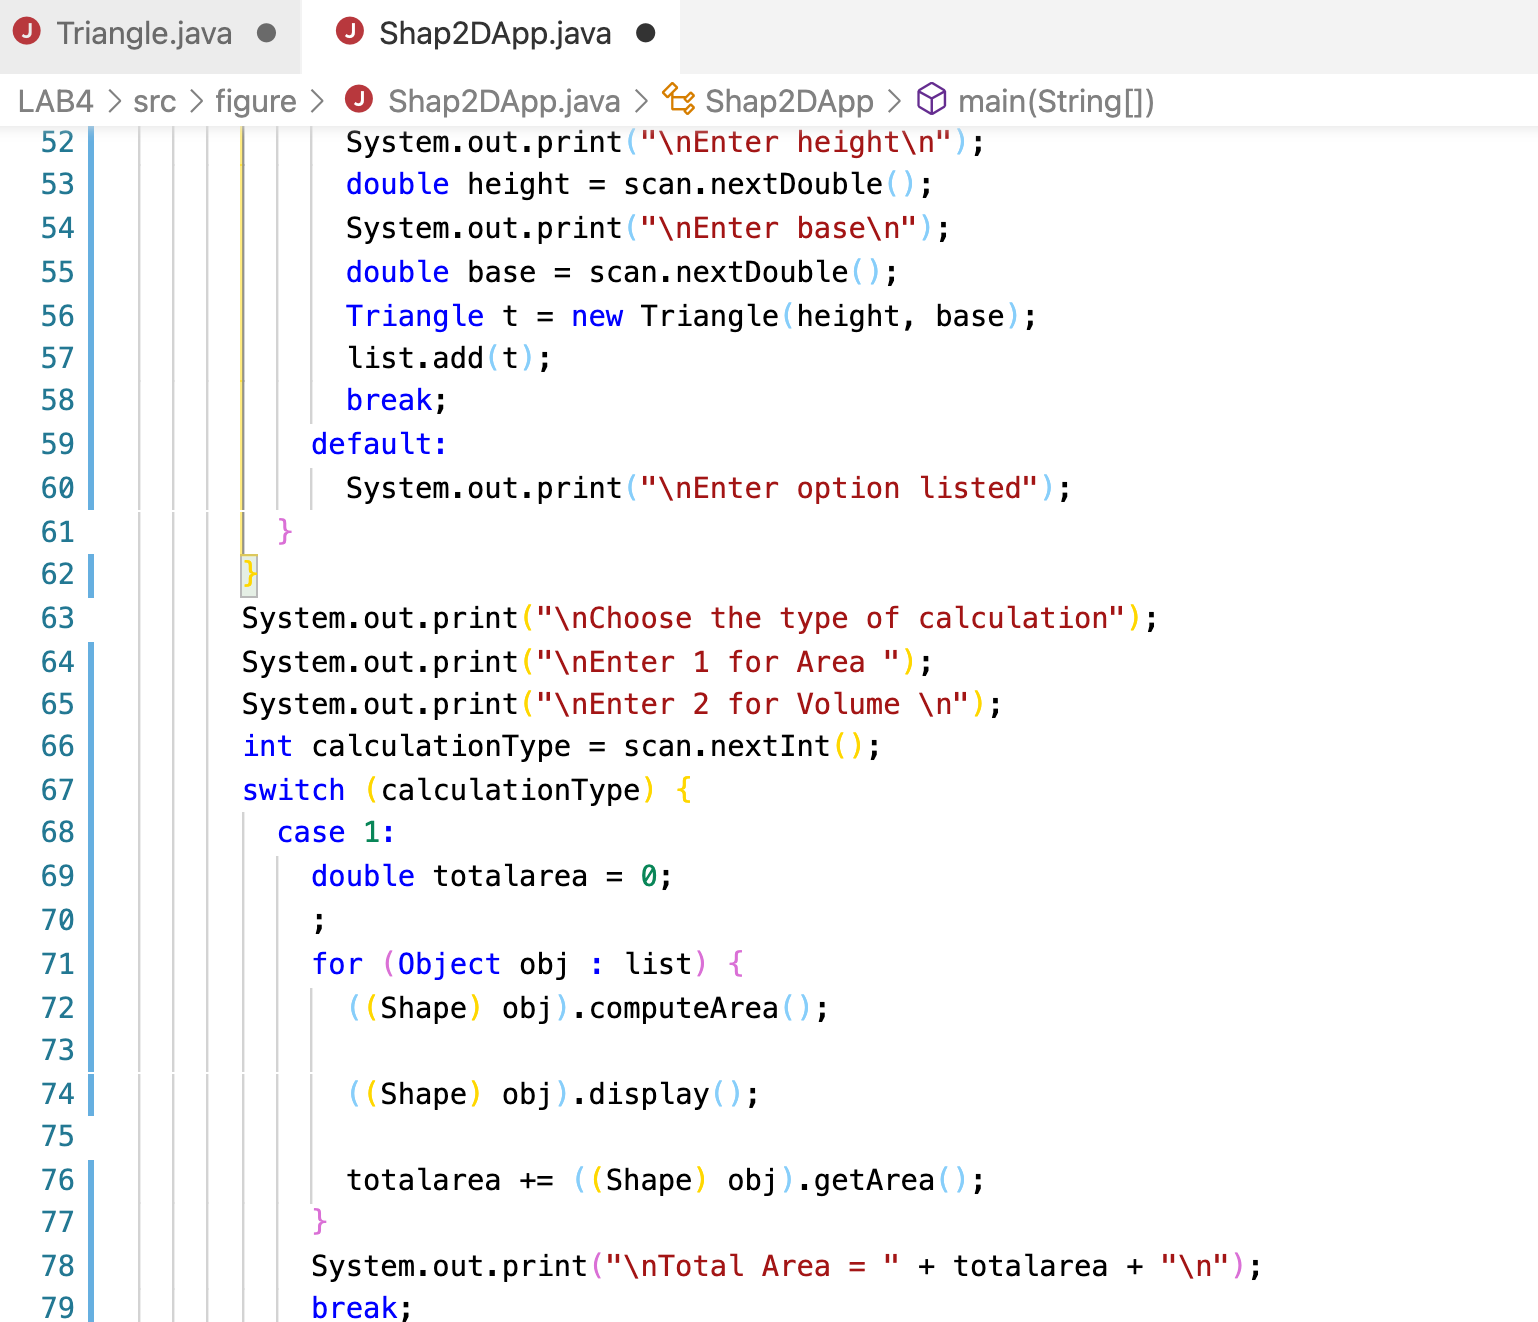
\includegraphics[scale=0.4]{z_shape2dapp3.png}
    
    \subsection{Shape3DApp.java}
    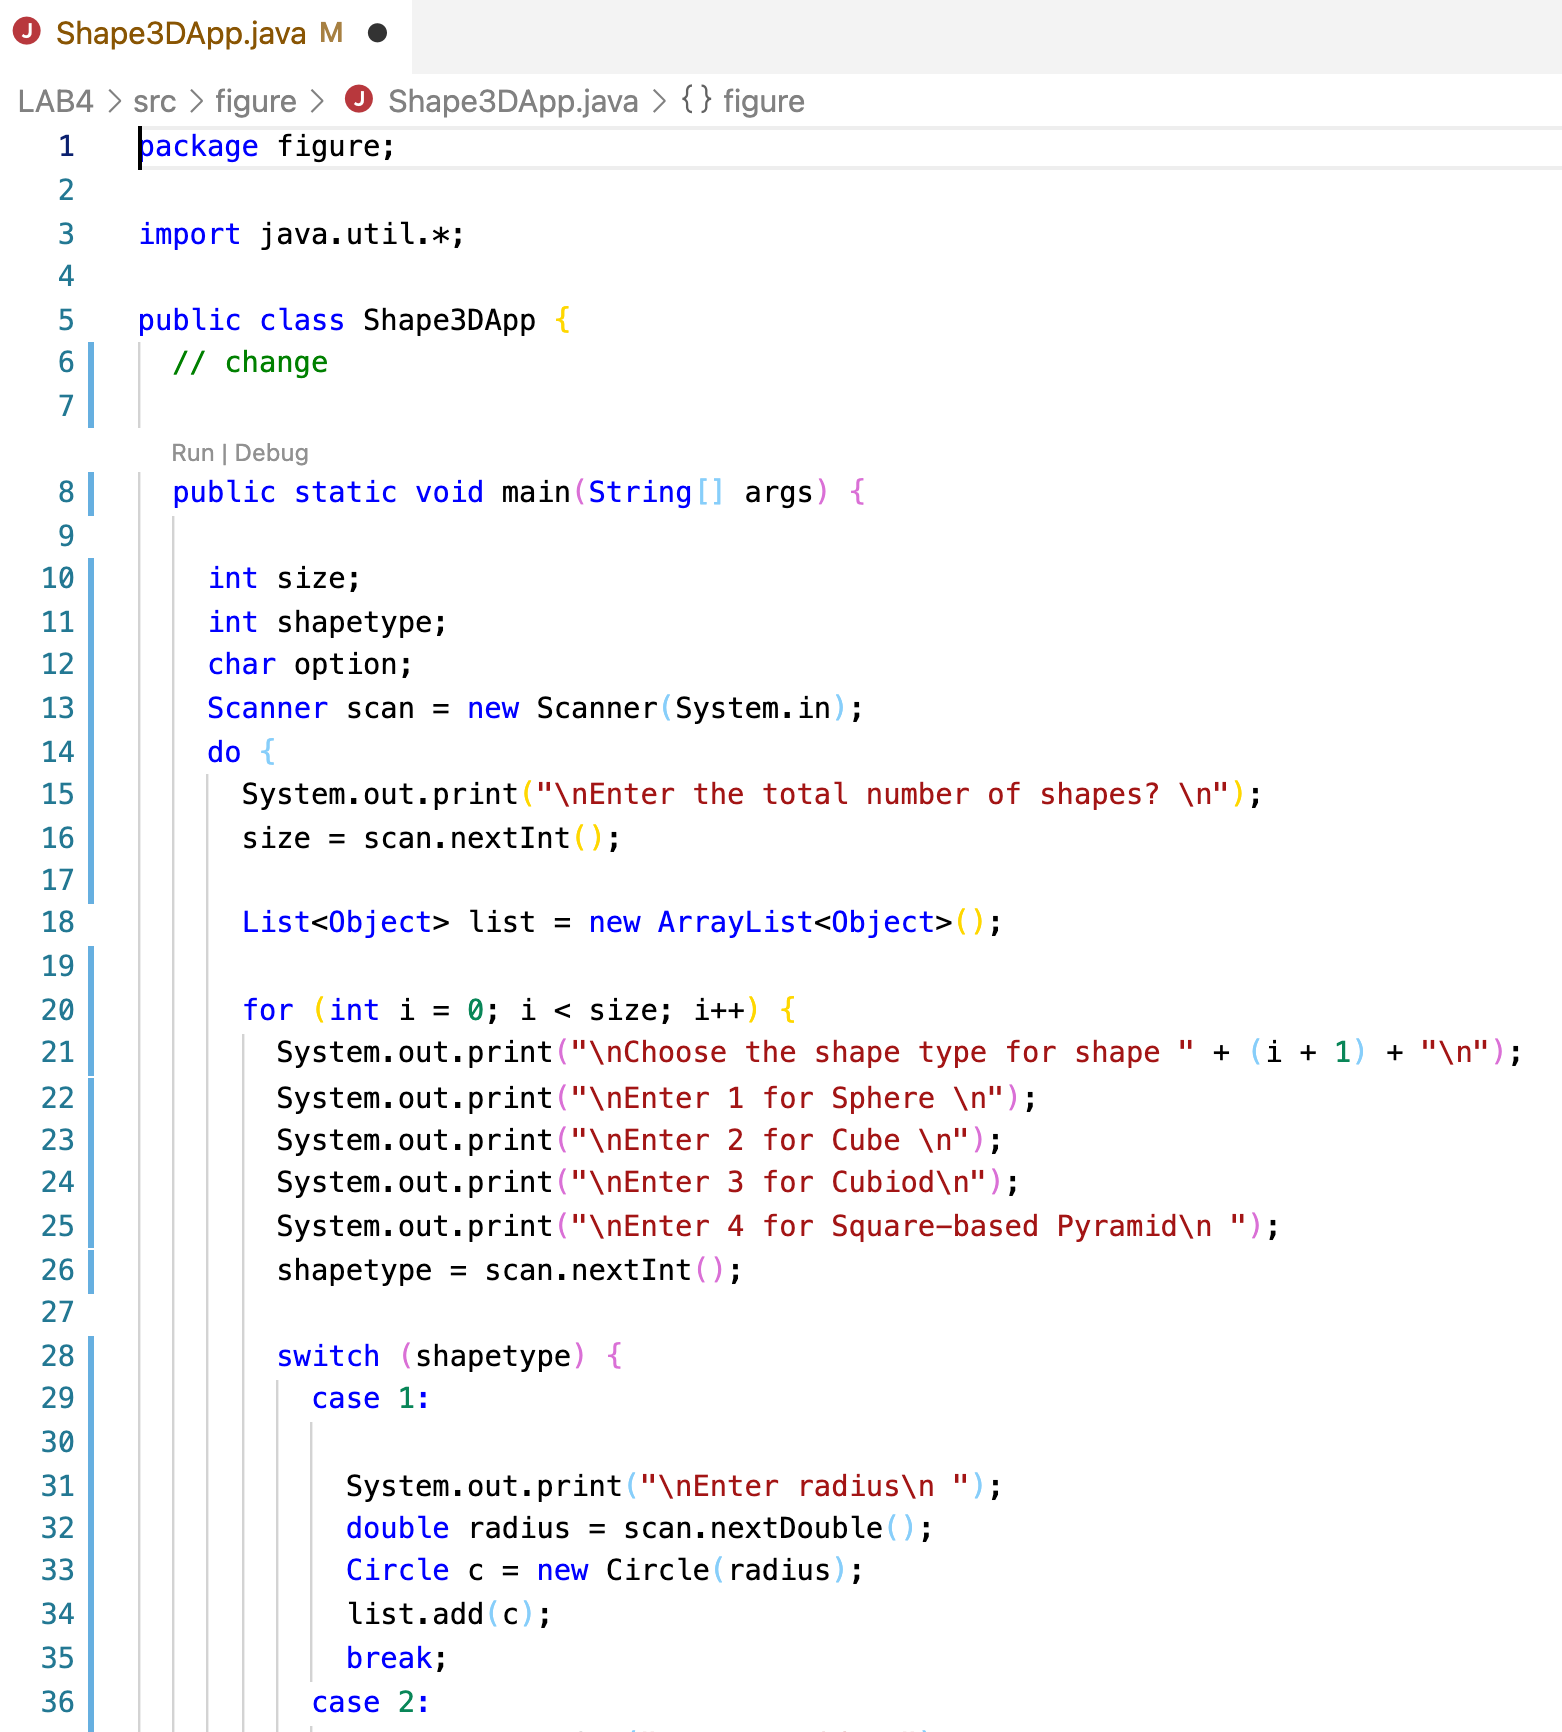
\includegraphics[scale=0.35]{z_shape3dapp1.png}
    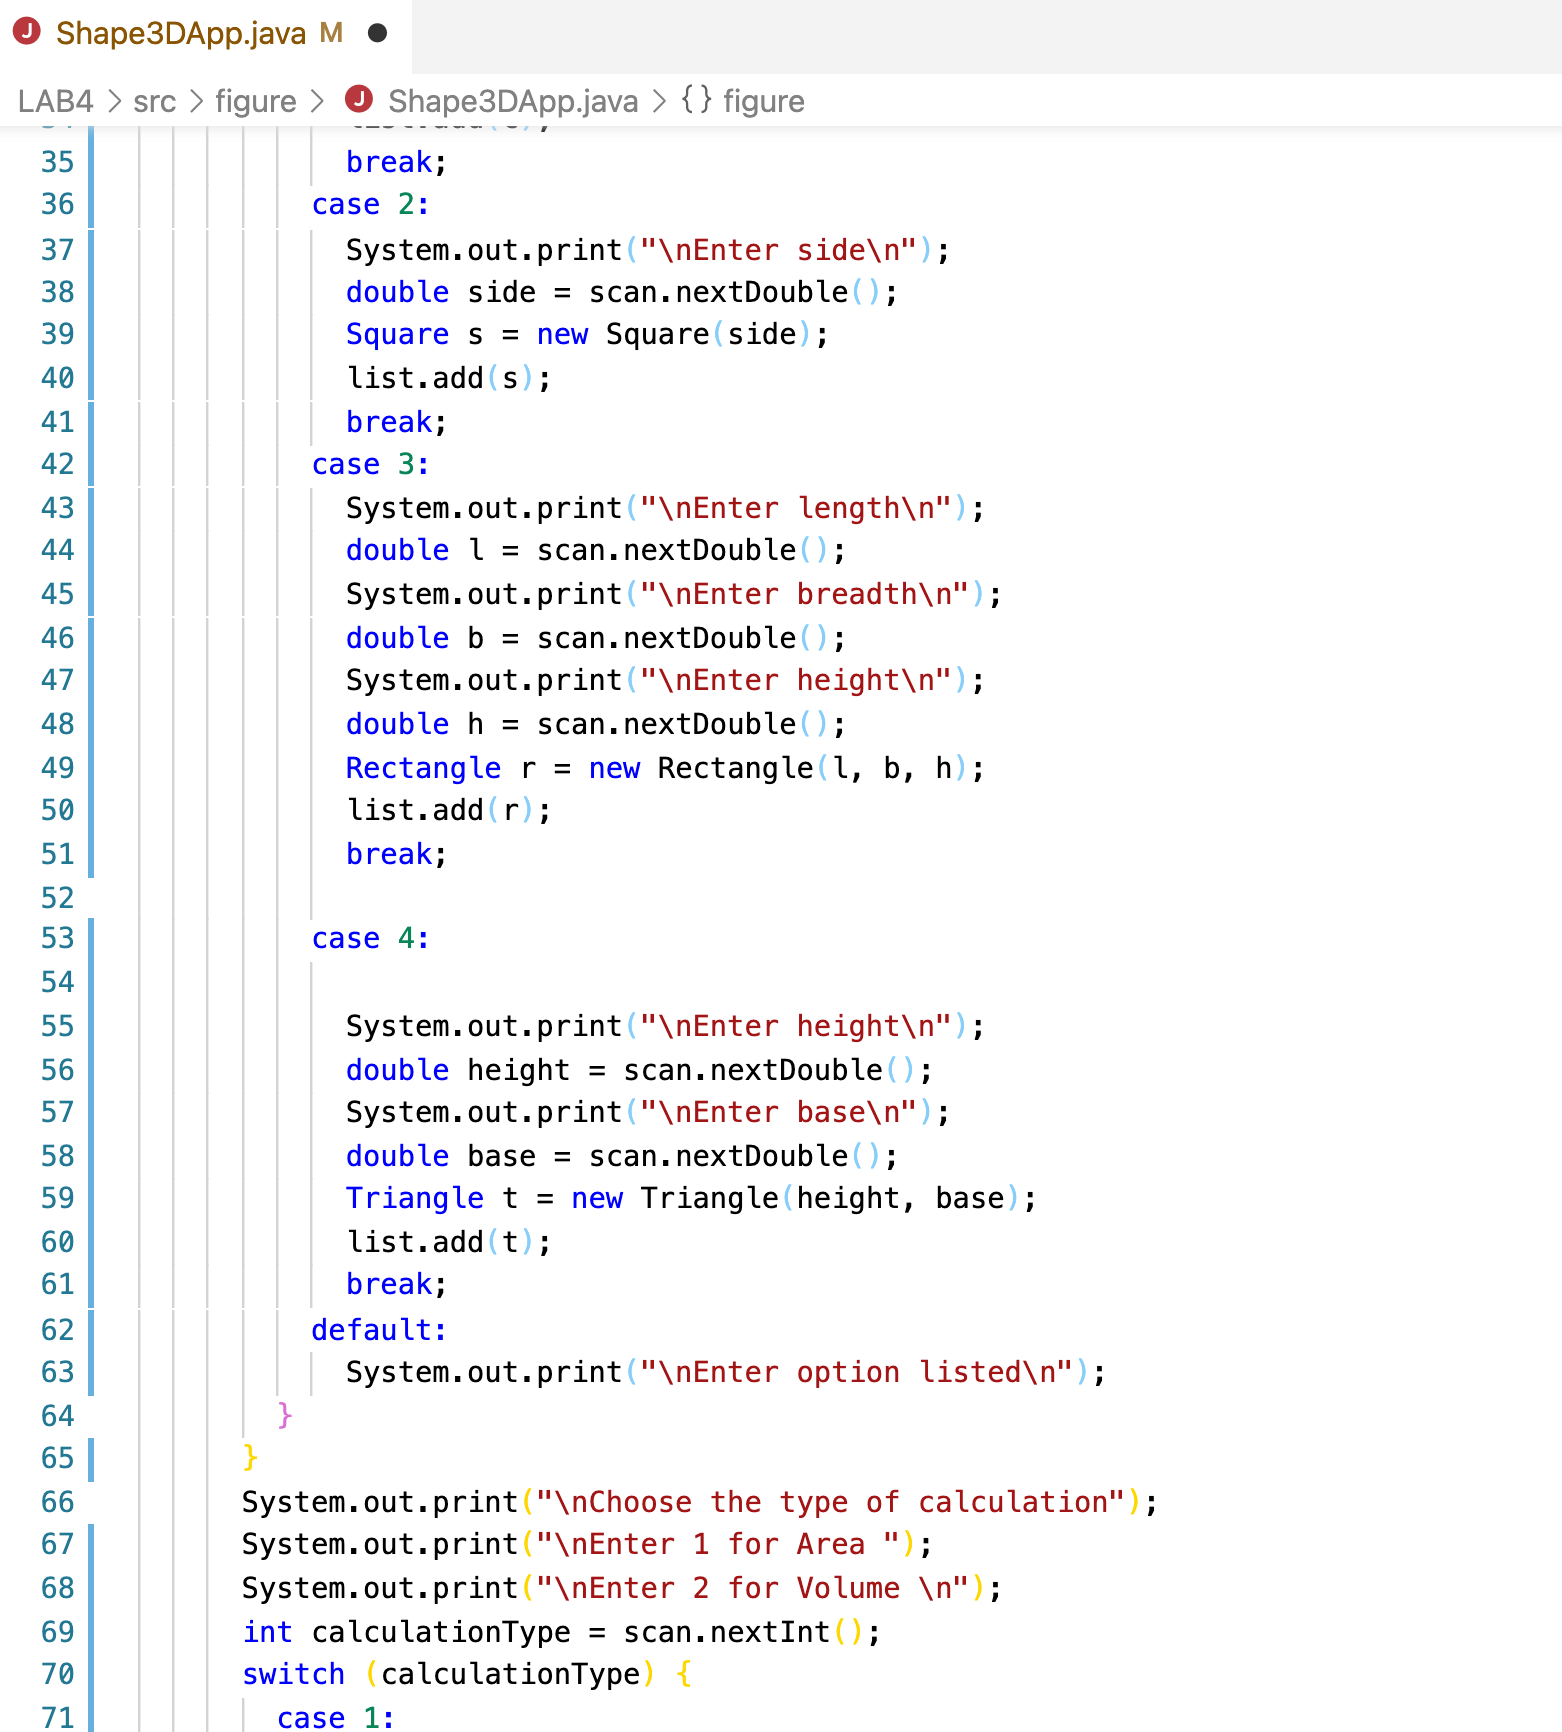
\includegraphics[scale=0.35]{z_shape3dapp2.png}
    
    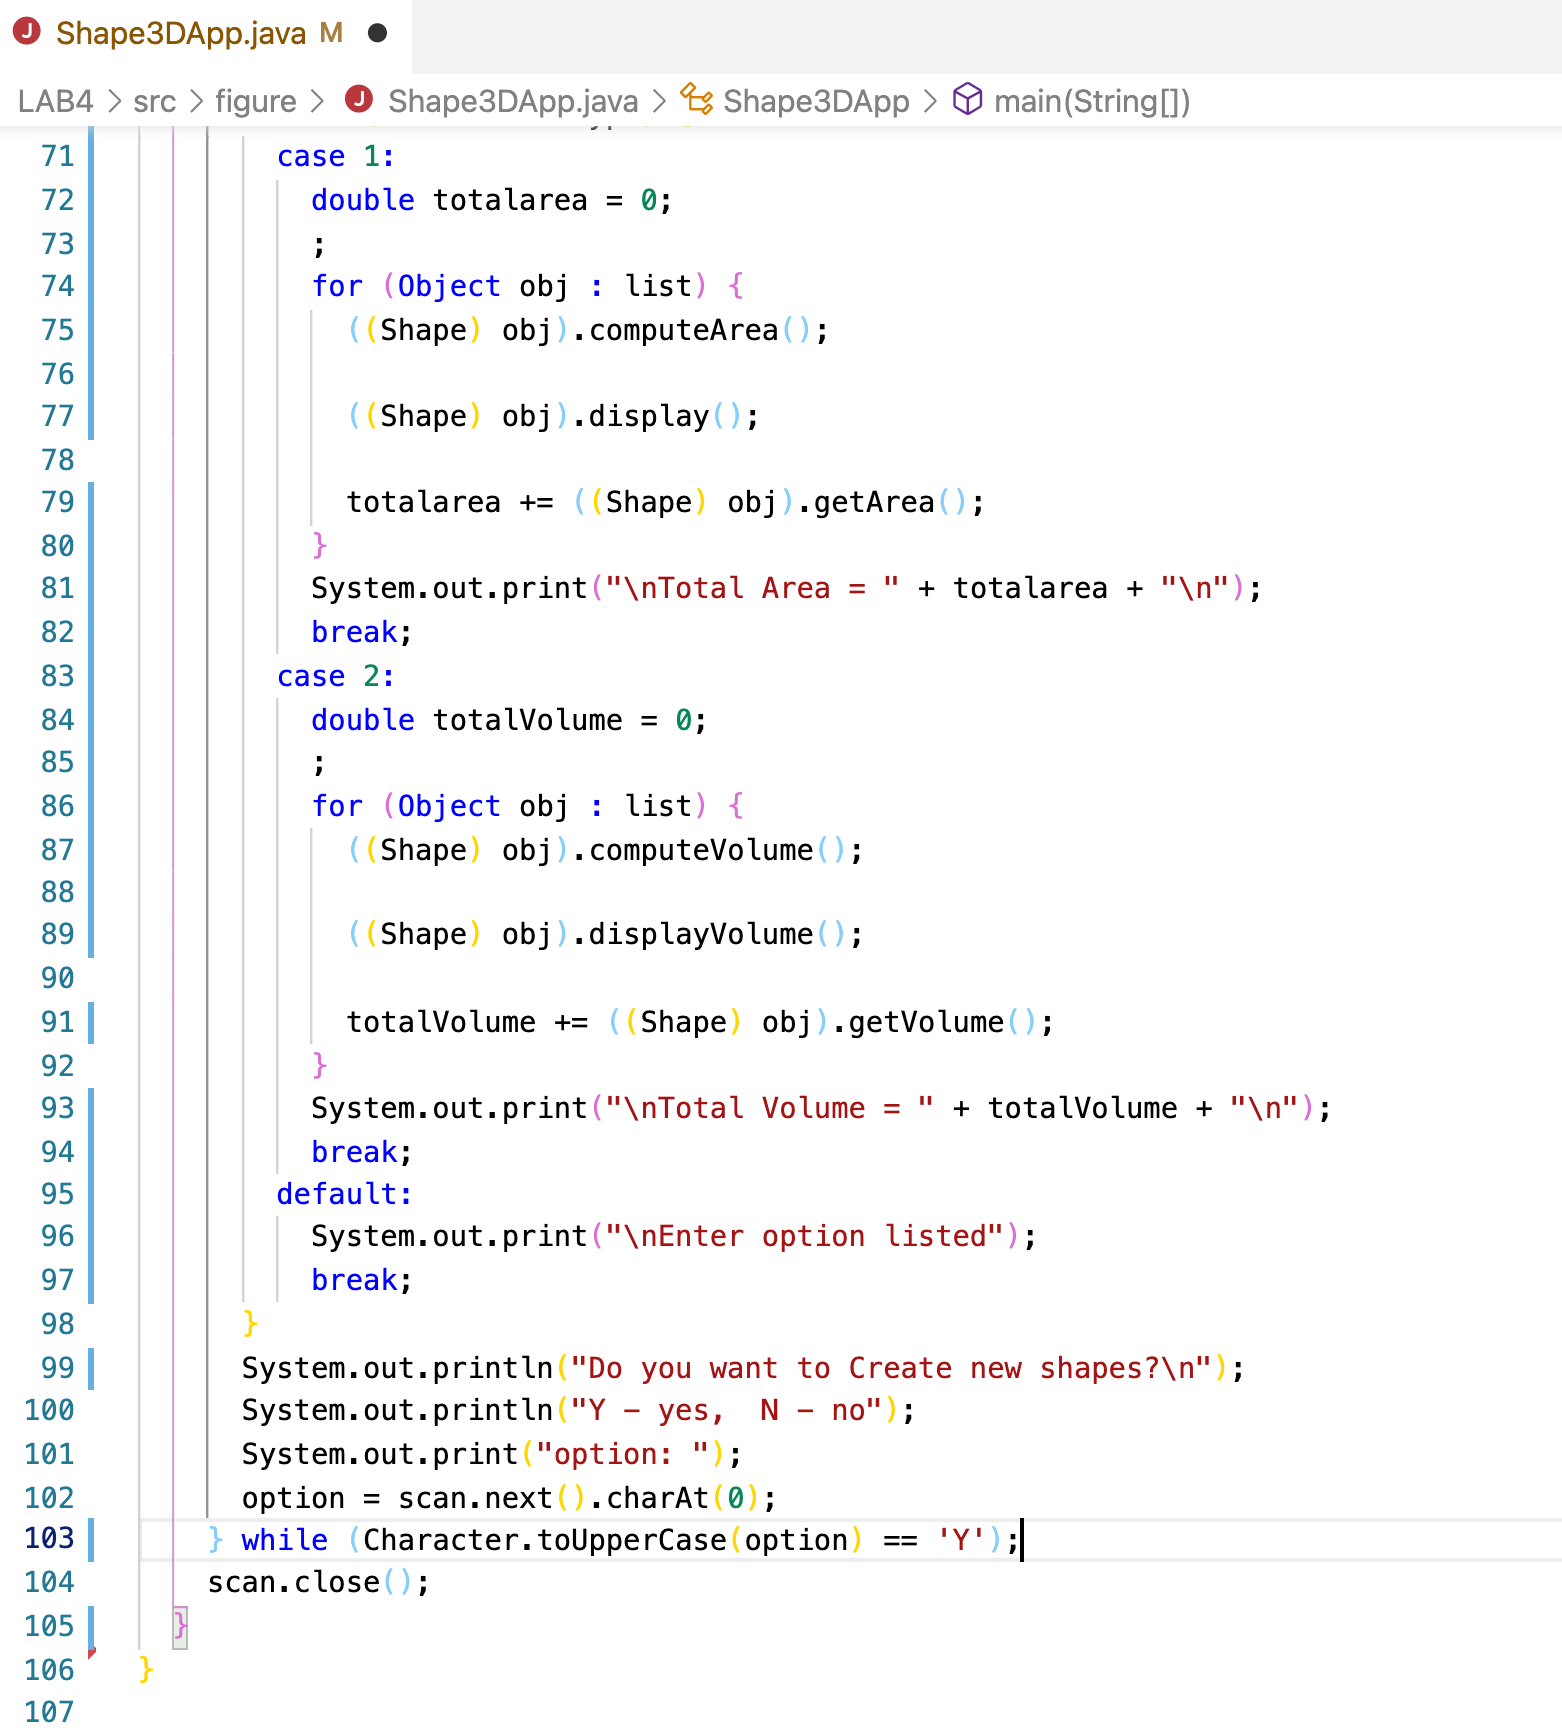
\includegraphics[scale=0.3]{z_shape3dapp3.png}
  
\subsection{Test Case for Area 2D figure}


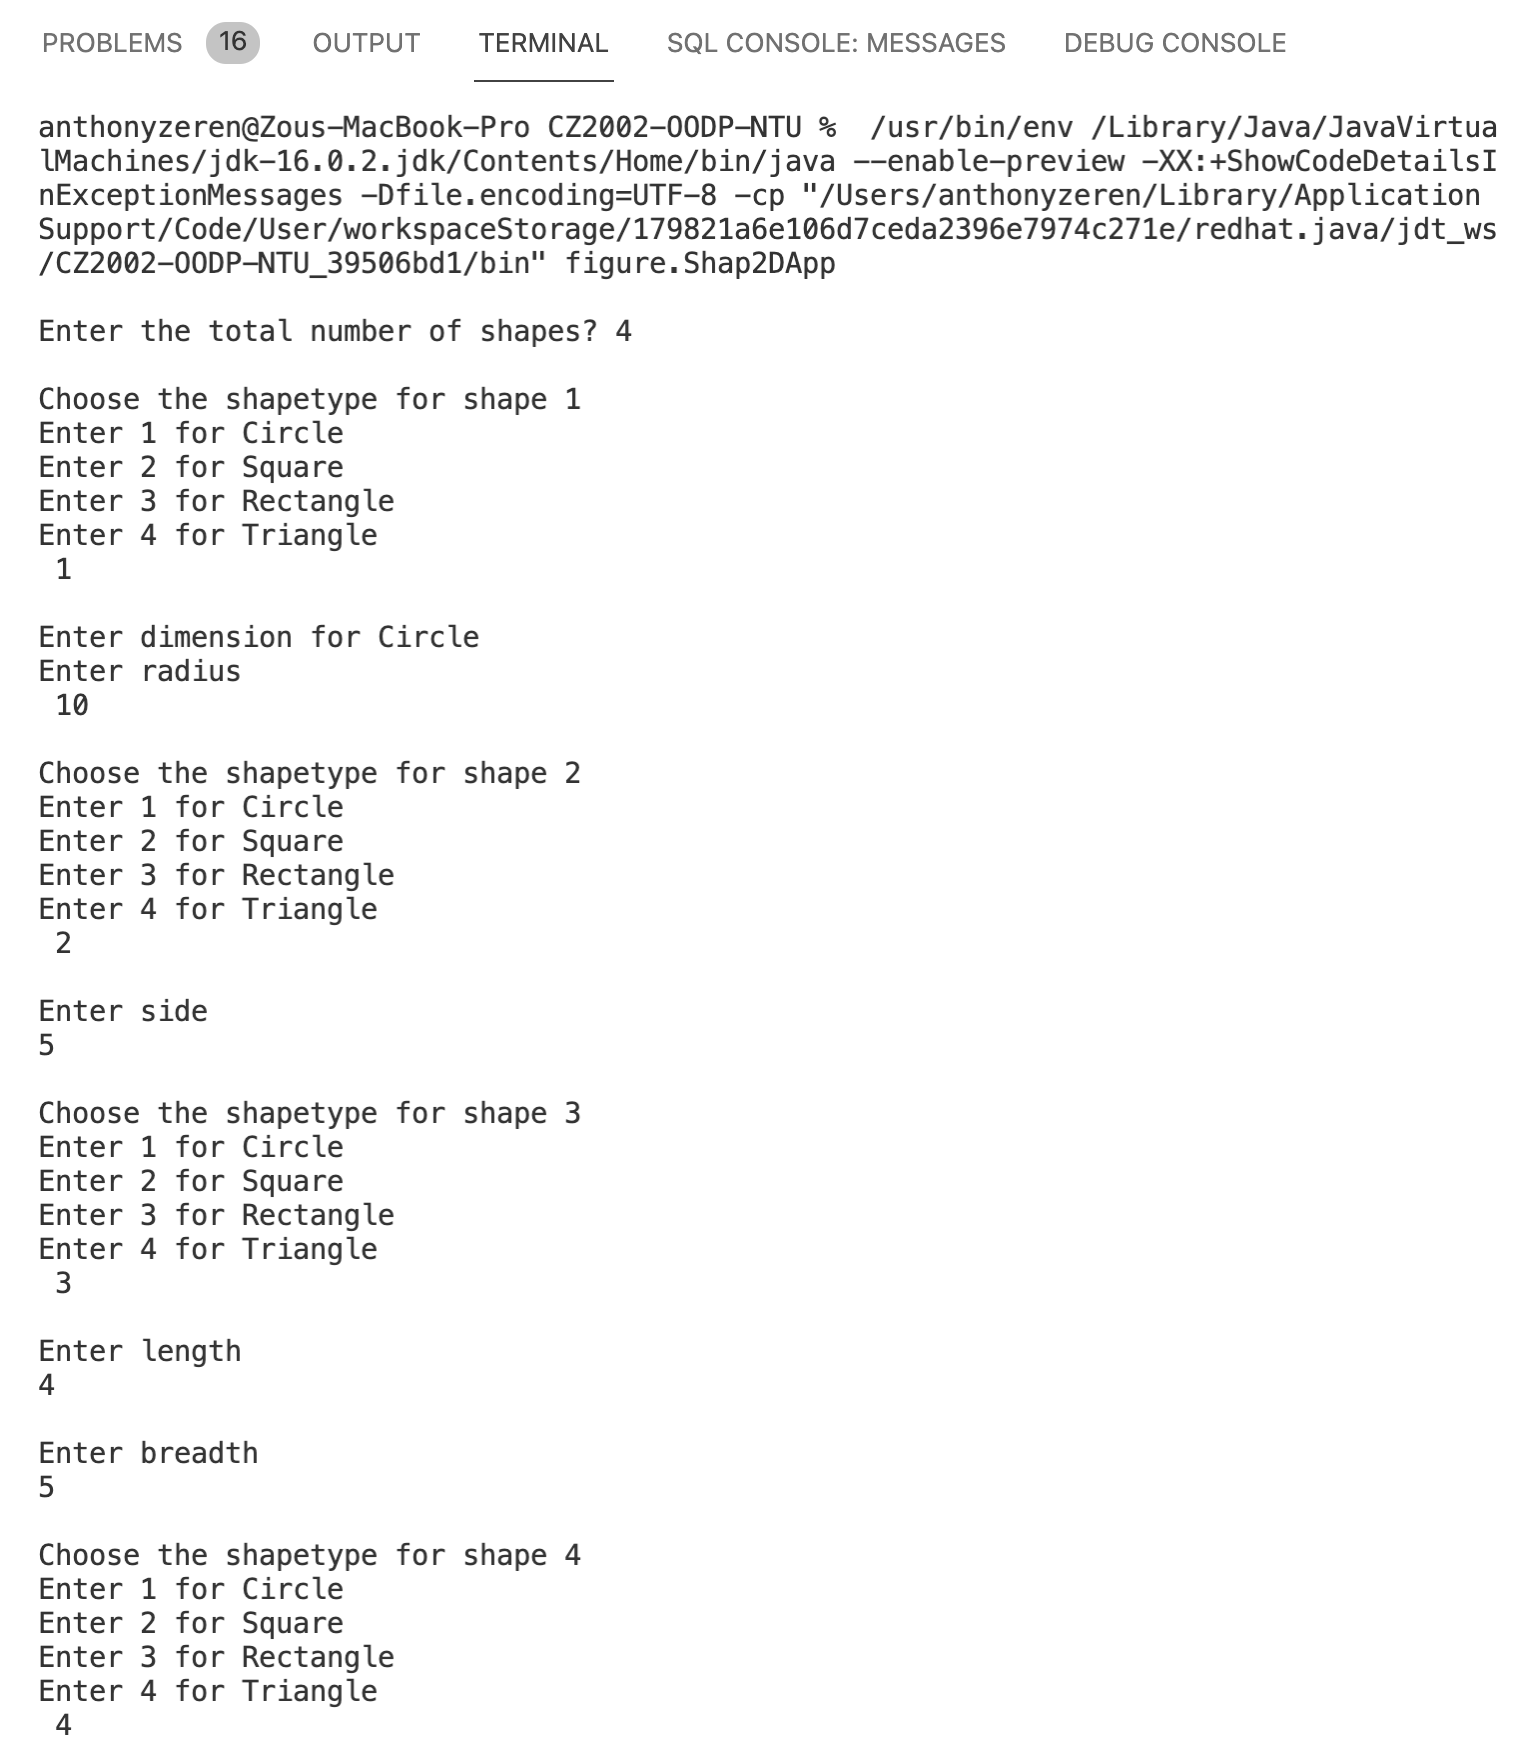
\includegraphics[scale=0.4]{tc2D1.png}
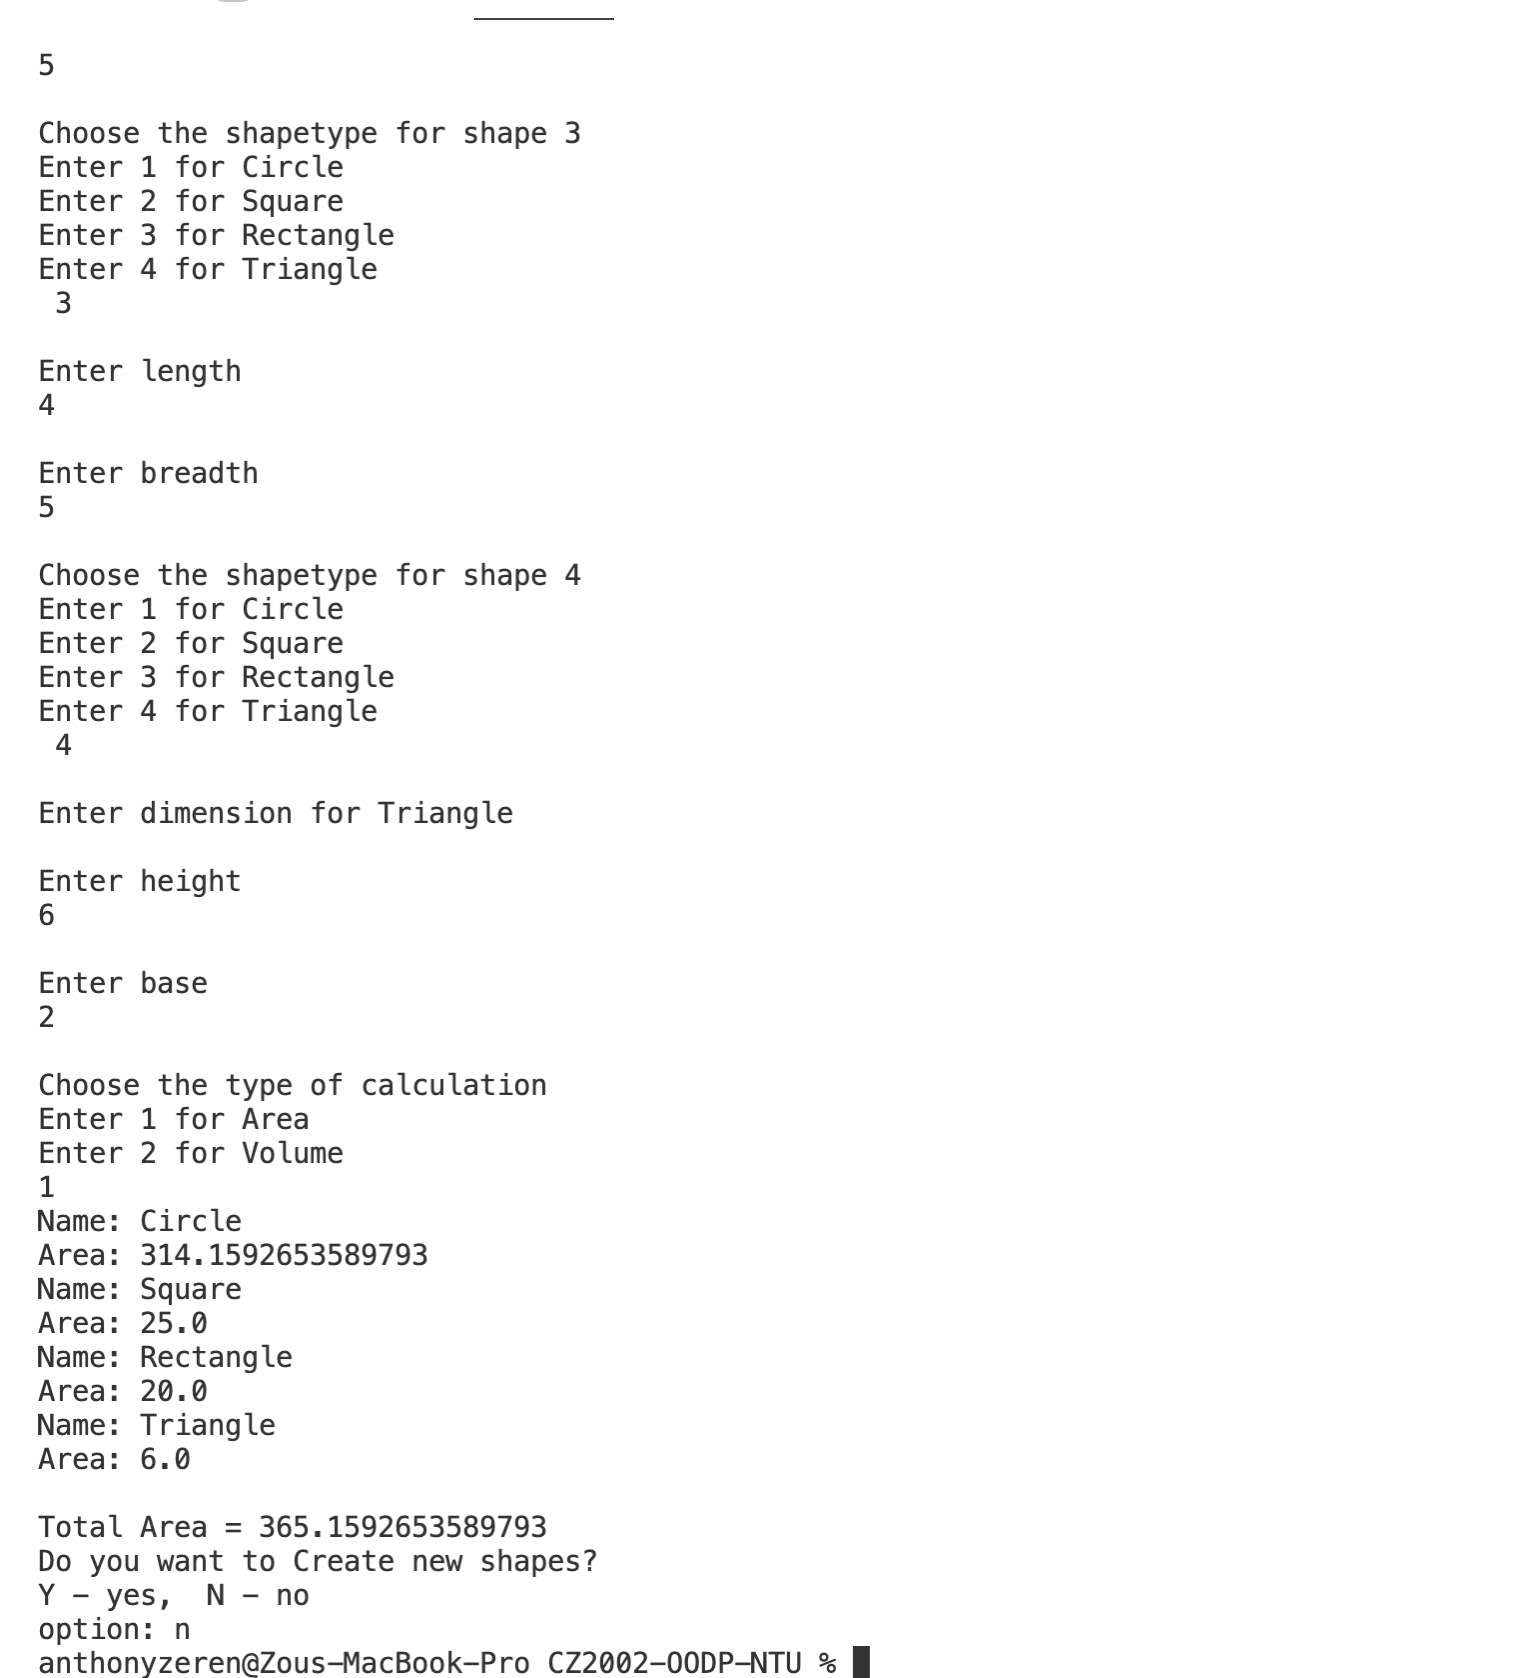
\includegraphics[scale=0.4]{tc2D2.png}
\subsection{Test Case for Area 3D figure}

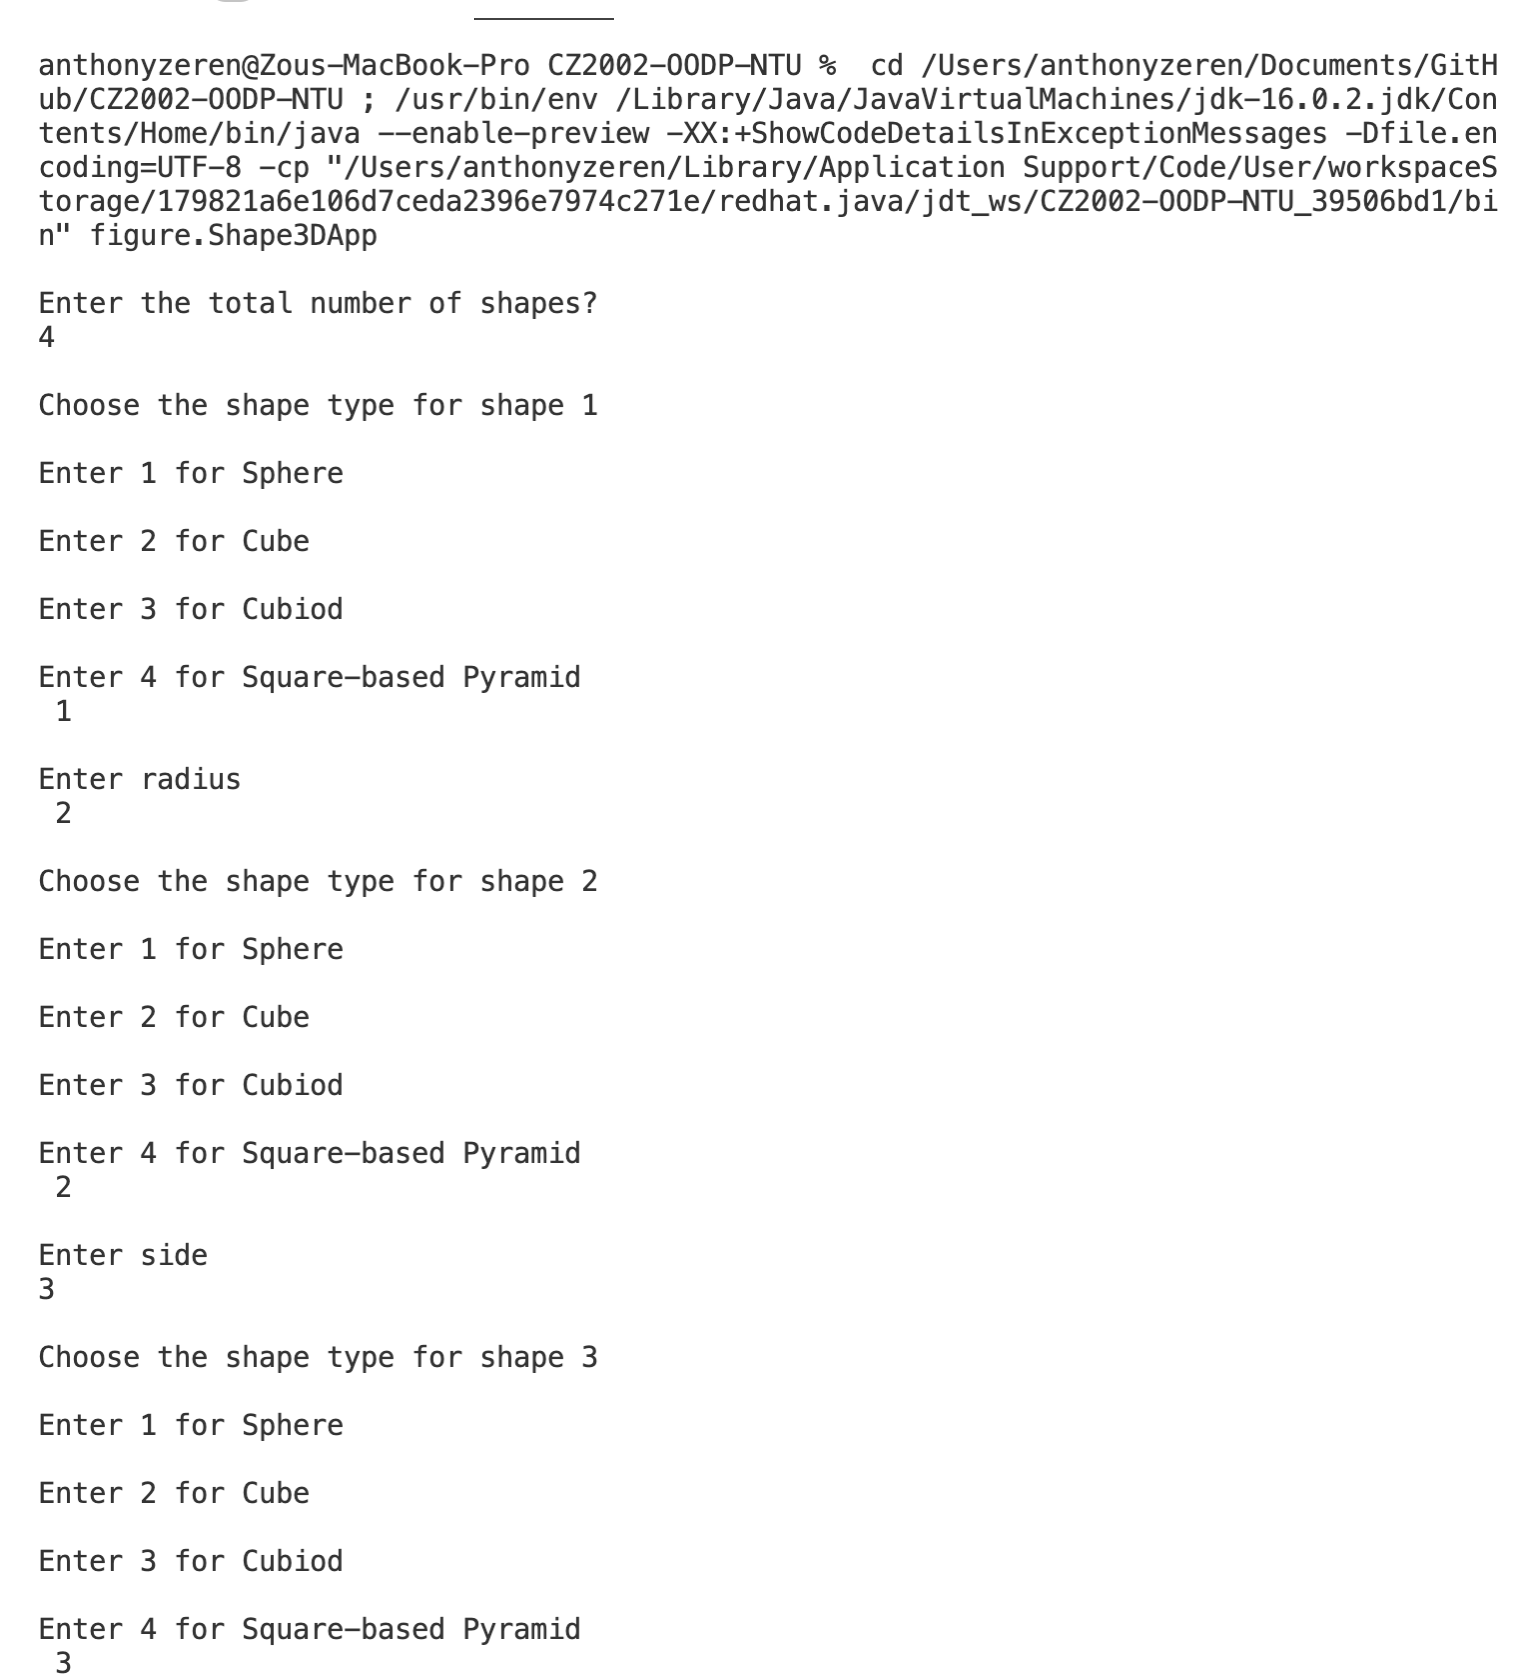
\includegraphics[scale=0.4]{tc3D1.png}
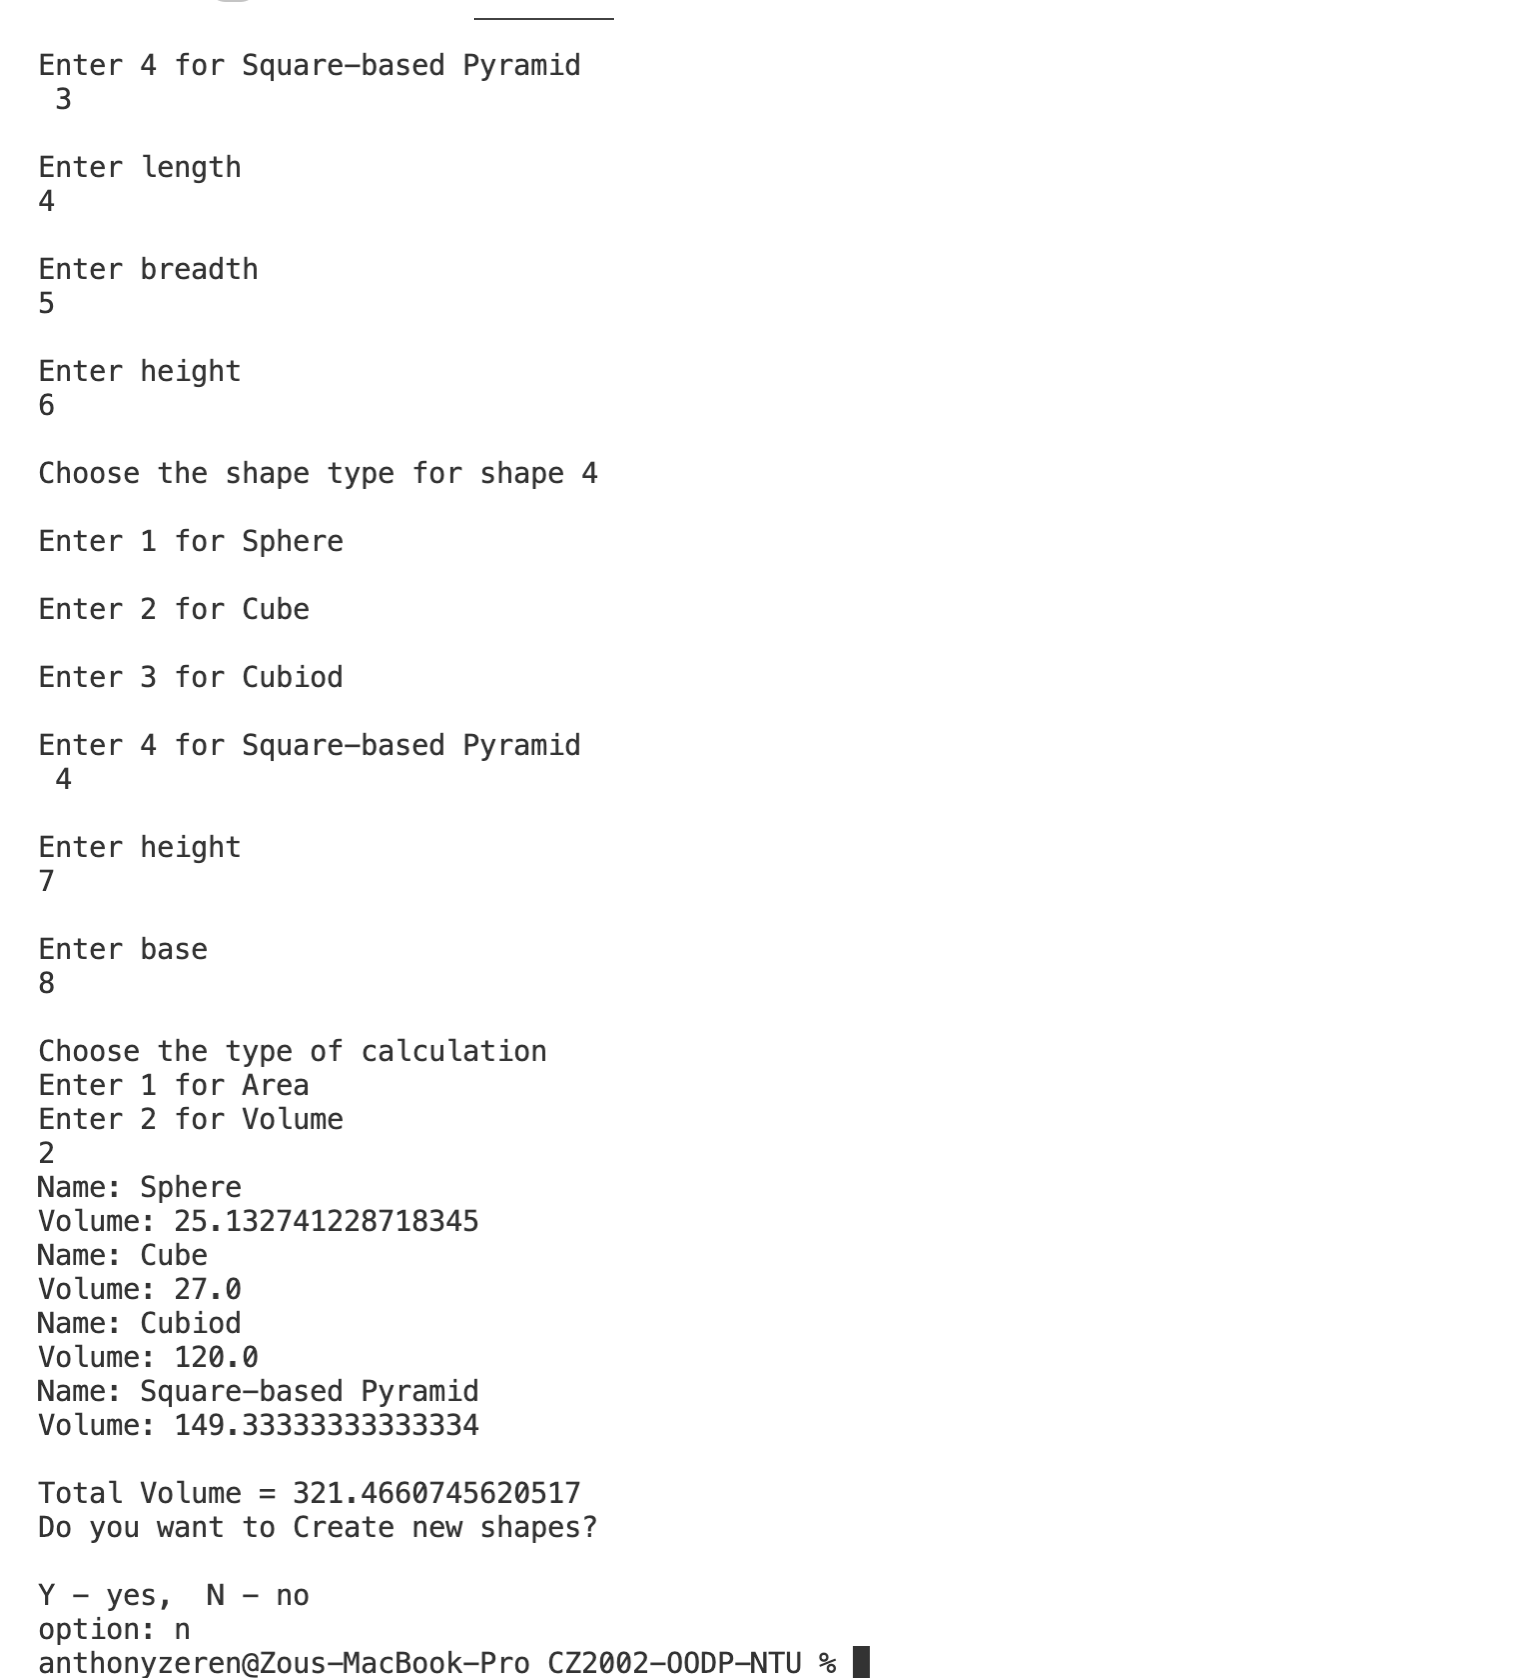
\includegraphics[scale=0.4]{tc3D2.png}


\end{document}